\documentclass[a4paper,12pt]{report}
%=====================================================
%  MÉMOIRE ESP / UCAD – STYLE COMPLET PROPRE
%=====================================================

%---------------- Encodage & langue ----------------
\usepackage[utf8]{inputenc}
\usepackage[T1]{fontenc}
\usepackage[french]{babel}
\frenchsetup{SmallCapsFigTabCaptions=false}
\usepackage{tabularx}
\usepackage{enumitem}

%---------------- Mise en page ----------------
\usepackage[a4paper,
  top=1.5cm, bottom=1.5cm,
  left=2.5cm, right=2cm]{geometry}

%---------------- Couleurs ----------------
\usepackage[dvipsnames,svgnames,x11names]{xcolor}

\definecolor{bleuESP}{RGB}{0,32,96}
\definecolor{orangeESP}{RGB}{192,80,77}
\definecolor{grisCadre}{RGB}{210,210,210}

%---------------- Graphiques ----------------
\usepackage{graphicx}
\usepackage{float}
\usepackage{tikz}
\usetikzlibrary{calc}
\usepackage{eso-pic}
\usepackage{url}

%---------------- Typographie ----------------
\usepackage{lmodern}
\usepackage{microtype}
\usepackage{ulem}
\normalem

%---------------- Table des matières ----------------
\usepackage[titles]{tocloft}

%=====================================================
%  NOMS NATIFS → style chapter* automatique
%=====================================================
\renewcommand{\contentsname}{Table des matières}
\renewcommand{\listfigurename}{Liste des figures}
\renewcommand{\listtablename}{Liste des tableaux}

%=====================================================
%  TITRES CHAPITRES
%=====================================================
\usepackage{titlesec}
\renewcommand{\thesection}{\Roman{section}}
\renewcommand{\thesubsection}{\thesection.\arabic{subsection}}
\setcounter{secnumdepth}{3}

\titleformat{\chapter}[display]
  {\bfseries\Huge\color{bleuESP}}
  {\filleft\Large\chaptername\ \thechapter}
  {1ex}
  {\titlerule[1pt]\vspace{1ex}\filright}
  [\vspace{1ex}\titlerule]

\titlespacing*{\chapter}{0pt}{-10pt}{25pt}

\titleformat{\section}
  {\bfseries\Large\color{bleuESP}}
  {\thesection}{1em}{}

\titleformat{\subsection}
  {\bfseries\normalsize\color{bleuESP}}
  {\thesubsection}{1em}{}

\titlespacing*{\section}{0pt}{10pt}{5pt}
\titlespacing*{\subsection}{0pt}{8pt}{4pt}

%=====================================================
%  EN-TÊTES / PIEDS DE PAGE
%=====================================================
\usepackage{fancyhdr}

\setlength{\headheight}{15pt}
\pagestyle{fancy}
\fancyhf{}

\renewcommand{\headrulewidth}{0.4pt}

\fancyhead[L]{\small\textit{\leftmark}}
\fancyhead[R]{\small\textit{ESP – UCAD}}
\fancyfoot[C]{\thepage}

%=====================================================
%  BOÎTES (optionnel)
%=====================================================
\usepackage{tcolorbox}
\tcbuselibrary{skins,breakable}

\newtcolorbox{boitesujet}{
  enhanced,
  colback=white,
  colframe=bleuESP,
  boxrule=1pt,
  arc=3pt,
  left=5pt,
  right=5pt,
  top=5pt,
  bottom=5pt
}

\newtcolorbox{boitestage}{
  enhanced,
  colback=white,
  colframe=bleuESP,
  boxrule=0.8pt,
  arc=3pt,
  left=5pt,
  right=5pt,
  top=5pt,
  bottom=5pt
}

\newtcolorbox{emplacementcapture}[1]{
  enhanced,
  colback=gray!3,
  colframe=grisCadre,
  boxrule=0.8pt,
  arc=2pt,
  height=5.2cm,
  valign=center,
  halign=center,
  fonttitle=\bfseries\small,
  title={#1},
  coltitle=bleuESP,
  colbacktitle=gray!8,
  boxed title style={boxrule=0pt,arc=0pt},
  attach boxed title to top center={yshift=-2mm},
  left=8pt,
  right=8pt,
  top=12pt,
  bottom=8pt
}

%=====================================================
%  CADRE AUTOMATIQUE AUTOUR DES FIGURES
%=====================================================
\usepackage{caption}

% Cadre gris clair autour des images
\setlength{\fboxsep}{6pt}      % espace entre image et cadre
\setlength{\fboxrule}{0.8pt}   % épaisseur du cadre

% Encadrement automatique de toutes les figures
% removed for pandoc
% removed fcolorbox wrapper for pandoc

% Style des légendes
\captionsetup{
  font=small,
  labelfont=bf,
  labelsep=period
}

%=====================================================
%  LIENS CLIQUABLES DANS LE PDF
%=====================================================
\usepackage[
  hidelinks,
  linktoc=all,
  bookmarksnumbered=true,
  bookmarksopen=true
]{hyperref}

%=====================================================
\begin{document}
\hypersetup{pageanchor=false}

%=====================================================
%  ██  PAGE DE GARDE  ██
%=====================================================
\thispagestyle{empty}

\AddToShipoutPictureBG*{%
  \begin{tikzpicture}[remember picture, overlay]
    % Ligne verticale gauche (bleue)
    \draw[bleuESP, line width=3pt]
      ($(current page.north west)+(1.35cm,-1cm)$)
      -- ($(current page.south west)+(1.35cm,1.6cm)$);
    % Ligne verticale droite (orange)
    \draw[orangeESP, line width=2pt]
      ($(current page.north east)+(-1.1cm,-1cm)$)
      -- ($(current page.south east)+(-1.1cm,1.6cm)$);
    % Petit carré bas gauche
    \draw[bleuESP, line width=2pt]
      ($(current page.south west)+(1.1cm,1.6cm)$)
      rectangle ++(0.5cm,0.5cm);
    % Petit carré bas droite
    \draw[orangeESP, line width=2pt]
      ($(current page.south east)+(-1.35cm,1.6cm)$)
      rectangle ++(0.5cm,0.5cm);
  \end{tikzpicture}%
}

\begin{center}
  \oldincludegraphics[height=1.4cm]{images/page-de-garde/drapeau_senegal.png}\\[0.15cm]
  % Titre université avec soulignement rouge (style image 2)
  {\Large\bfseries UNIVERSITE CHEIKH ANTA DIOP DE DAKAR}\\[-0.05cm]
  {\color{red}\rule{\linewidth}{1.5pt}}\\[0.2cm]
  \oldincludegraphics[height=2cm]{images/page-de-garde/logo_ucad.png}\\[0.05cm]
  {\small\bfseries ECOLE SUPERIEURE POLYTECHNIQUE}\\[0.15cm]
  {\color{bleuESP}\rule{\linewidth}{1pt}}\\[0.1cm]
  {\color{bleuESP}\bfseries\itshape\uline{DEPARTEMENT GENIE INFORMATIQUE}}\\[0.05cm]
  {\color{bleuESP}\rule{\linewidth}{1pt}}\\[0.2cm]

  % Boîte MEMOIRE — contour bleu, fond blanc (style image 2)
  \begin{tcolorbox}[
    enhanced,
    arc=4pt, boxrule=1.5pt,
    left=6pt, right=6pt, top=5pt, bottom=5pt,
    colback=white, colframe=bleuESP,
    halign=center,
  ]
    \textbf{\large MEMOIRE DE FIN DE CYCLE}\\[0.15cm]
    \textbf{Pour l'obtention du :}\\[0.1cm]
    \textbf{DIPLOME D'INGENIEUR DE CONCEPTION EN GENIE INFORMATIQUE}\\[0.1cm]
    \textbf{OPTION : INFORMATIQUE}
  \end{tcolorbox}
  \vspace{0.2cm}

  % Boîte SUJET — contour bleu, fond blanc, texte noir (style image 2)
  \begin{tcolorbox}[
    enhanced,
    arc=4pt,
    boxrule=1.5pt,
    colback=white,
    colframe=bleuESP,
    left=6pt,
    right=6pt,
    top=6pt,
    bottom=6pt,
    halign=center,
  ]
    {\large\bfseries\uline{SUJET :}}\\[0.2cm]
    {\itshape
    Conception d'un système d'information bancaire intelligent : cas des modules
    Relation Client et SGI (Société de Gestion et d'Intermédiation).}
  \end{tcolorbox}


\begin{boitestage}
    \noindent
    \textbf{Lieu de stage :} \textcolor{orangeESP}{\textbf{INNOV4AFRICA}}
    \hfill
    \textbf{Période de stage :} \textcolor{orangeESP}{\textbf{15/08/2025 -- 30/06/2026}}
    \vspace{0.05cm}
    \begin{center}
        \oldincludegraphics[height=3.2cm]{images/page-de-garde/innov4africa_logo.jpg}
    \end{center}
    \vspace{-0.35cm}
\end{boitestage}
\end{center}



\noindent\textbf{Présenté et soutenu par:}\quad Salif Biaye\\[0.15cm]
\textbf{\quad PROMOTION: 2026 \;--\; DATE DE SOUTENANCE: xx/07/2026}

 

\textcolor{bleuESP}{\textbf{MEMBRES DU JURY:}}

\vspace{0.15cm}
\noindent
\begin{tabular}{@{}p{4.5cm} p{5cm} p{4.5cm}@{}}
  \textcolor{bleuESP}{PRESIDENT}            & & \\[2pt]
  \textcolor{bleuESP}{RAPPORTEUR}           & & \\[2pt]
  \textcolor{bleuESP}{EXAMINATEUR}          & & \\[2pt]
  \textcolor{bleuESP}{ENCADRANT}            & Pr Ibrahima Fall  & Maître de conférences \\[2pt]
  \textcolor{bleuESP}{MAITRE DE STAGE}      & Khassoum WONE     & Ingénieur Informatique \\[2pt]
  \textcolor{bleuESP}{DIRECTEUR DE MEMOIRE} & Pr Ibrahima Fall  & Maître de conférences \\
\end{tabular}

\vfill

\begin{tcolorbox}[
  enhanced,
  arc=4pt, boxrule=1.5pt,
  left=6pt, right=6pt, top=5pt, bottom=5pt,
  colback=white, colframe=bleuESP,
  halign=center,
]
  
  \small Année universitaire : 2025 - 2026\\[0.1cm]
  
\end{tcolorbox}

\cleardoublepage


%=====================================================
%  ██  PAGE DE GARDE  ██
%=====================================================
\thispagestyle{empty}

\AddToShipoutPictureBG*{%
  \begin{tikzpicture}[remember picture, overlay]
    % Ligne verticale gauche (bleue)
    \draw[bleuESP, line width=3pt]
      ($(current page.north west)+(1.35cm,-1cm)$)
      -- ($(current page.south west)+(1.35cm,1.6cm)$);
    % Ligne verticale droite (orange)
    \draw[orangeESP, line width=2pt]
      ($(current page.north east)+(-1.1cm,-1cm)$)
      -- ($(current page.south east)+(-1.1cm,1.6cm)$);
    % Petit carré bas gauche
    \draw[bleuESP, line width=2pt]
      ($(current page.south west)+(1.1cm,1.6cm)$)
      rectangle ++(0.5cm,0.5cm);
    % Petit carré bas droite
    \draw[orangeESP, line width=2pt]
      ($(current page.south east)+(-1.35cm,1.6cm)$)
      rectangle ++(0.5cm,0.5cm);
  \end{tikzpicture}%
}

\begin{center}
  \oldincludegraphics[height=1.4cm]{images/page-de-garde/drapeau_senegal.png}\\[0.15cm]
  % Titre université avec soulignement rouge (style image 2)
  {\Large\bfseries UNIVERSITE CHEIKH ANTA DIOP DE DAKAR}\\[-0.05cm]
  {\color{red}\rule{\linewidth}{1.5pt}}\\[0.2cm]
  \oldincludegraphics[height=2cm]{images/page-de-garde/logo_ucad.png}\\[0.05cm]
  {\small\bfseries ECOLE SUPERIEURE POLYTECHNIQUE}\\[0.15cm]
  {\color{bleuESP}\rule{\linewidth}{1pt}}\\[0.1cm]
  {\color{bleuESP}\bfseries\itshape\uline{DEPARTEMENT GENIE INFORMATIQUE}}\\[0.05cm]
  {\color{bleuESP}\rule{\linewidth}{1pt}}\\[0.2cm]

  % Boîte MEMOIRE — contour bleu, fond blanc (style image 2)
  \begin{tcolorbox}[
    enhanced,
    arc=4pt, boxrule=1.5pt,
    left=6pt, right=6pt, top=5pt, bottom=5pt,
    colback=white, colframe=bleuESP,
    halign=center,
  ]
    \textbf{\large MEMOIRE DE FIN DE CYCLE}\\[0.15cm]
    \textbf{Pour l'obtention du :}\\[0.1cm]
    \textbf{DIPLOME D'INGENIEUR DE CONCEPTION EN GENIE INFORMATIQUE}\\[0.1cm]
    \textbf{OPTION : INFORMATIQUE}
  \end{tcolorbox}
  \vspace{0.2cm}

  % Boîte SUJET — contour bleu, fond blanc, texte noir (style image 2)
  \begin{tcolorbox}[
    enhanced,
    arc=4pt,
    boxrule=1.5pt,
    colback=white,
    colframe=bleuESP,
    left=6pt,
    right=6pt,
    top=6pt,
    bottom=6pt,
    halign=center,
  ]
    {\large\bfseries\uline{SUJET :}}\\[0.2cm]
    {\itshape
    Conception d'un système d'information bancaire intelligent : cas des modules
    Relation Client et SGI (Société de Gestion et d'Intermédiation).}
  \end{tcolorbox}


\begin{boitestage}
    \noindent
    \textbf{Lieu de stage :} \textcolor{orangeESP}{\textbf{INNOV4AFRICA}}
    \hfill
    \textbf{Période de stage :} \textcolor{orangeESP}{\textbf{15/08/2025 -- 30/06/2026}}
    \vspace{0.05cm}
    \begin{center}
        \oldincludegraphics[height=3.2cm]{images/page-de-garde/innov4africa_logo.jpg}
    \end{center}
    \vspace{-0.35cm}
\end{boitestage}
\end{center}



\noindent\textbf{Présenté et soutenu par:}\quad Salif Biaye\\[0.15cm]
\textbf{\quad PROMOTION: 2026 \;--\; DATE DE SOUTENANCE: xx/07/2026}

 

\textcolor{bleuESP}{\textbf{MEMBRES DU JURY:}}

\vspace{0.15cm}
\noindent
\begin{tabular}{@{}p{4.5cm} p{5cm} p{4.5cm}@{}}
  \textcolor{bleuESP}{PRESIDENT}            & & \\[2pt]
  \textcolor{bleuESP}{RAPPORTEUR}           & & \\[2pt]
  \textcolor{bleuESP}{EXAMINATEUR}          & & \\[2pt]
  \textcolor{bleuESP}{ENCADRANT}            & Pr Ibrahima Fall  & Maître de conférences \\[2pt]
  \textcolor{bleuESP}{MAITRE DE STAGE}      & Khassoum WONE     & Ingénieur Informatique \\[2pt]
  \textcolor{bleuESP}{DIRECTEUR DE MEMOIRE} & Pr Ibrahima Fall  & Maître de conférences \\
\end{tabular}

\vfill

\begin{tcolorbox}[
  enhanced,
  arc=4pt, boxrule=1.5pt,
  left=6pt, right=6pt, top=5pt, bottom=5pt,
  colback=white, colframe=bleuESP,
  halign=center,
]
  
  \small Année universitaire : 2025 - 2026\\[0.1cm]
  
\end{tcolorbox}

\cleardoublepage

\hypersetup{pageanchor=true}
%=====================================================
%  ██  PRÉLUDE  ██
%  Numérotation romaine repart à i
%=====================================================
\pagenumbering{roman}
\setcounter{page}{1}

% ─────────────────────────────────────────────────
%  DÉDICACES 
% ─────────────────────────────────────────────────

\chapter*{Dédicaces}
\phantomsection
\addcontentsline{toc}{chapter}{Dédicaces}
\markboth{Dédicaces}{Dédicaces}

\vspace{1cm}

\begin{center}
\begin{minipage}{0.9\textwidth}

\textit{Au nom d'ALLAH le clément et le miséricordieux}\\[0.5cm]
\textit{Je tiens à dédier ce modeste travail}

\vspace{0.8cm}

\begin{itemize}
  \setlength\itemsep{0.5em}

  \item À mes très chers parents, à ma mère \textbf{Fatimatou Bineta Dia}
  pour son amour inconditionnel, son soutien indéfectible et ses prières
  tout au long de mon parcours, et à la mémoire de mon père
  \textbf{Mouhamadou Lamine Biaye}, que ALLAH lui accorde Sa miséricorde
  et l’accueille en Son paradis.

  \item À mon frère \textbf{Mouhamad Hamza Biaye} et à ma sœur
  \textbf{Adja Mariama Biaye}, pour leur affection et leurs encouragements.

  \item À toute ma famille, du côté maternel comme paternel, pour leur soutien constant.

  \item À mes cousins et cousines pour leur présence et leur bienveillance.

  \item À mes camarades de promotion de l’ESP pour la solidarité et les efforts partagés.

  \item À mes amis pour leur amitié sincère et précieuse.

  \item À tous ceux qui ont contribué, de près ou de loin, à ce travail.

\end{itemize}

\end{minipage}
\end{center}

\cleardoublepage

% ─────────────────────────────────────────────────
%  REMERCIEMENTS
% ─────────────────────────────────────────────────
\chapter*{Remerciements}
\phantomsection
\addcontentsline{toc}{chapter}{Remerciements}
\markboth{Remerciements}{Remerciements}

Mes remerciements vont d'abord à \textbf{Pr Ibrahima Fall}, mon encadrant et
directeur de mémoire, pour sa disponibilité, ses précieux conseils et son
accompagnement tout au long de ce travail.

Je remercie également \textbf{Khassoum WONE}, mon maître de stage chez
INNOV4AFRICA, pour l'accueil chaleureux et l'encadrement professionnel.

Je remercie enfin l'ensemble du corps enseignant du Département Génie
Informatique de l'ESP pour la qualité de la formation dispensée.

\cleardoublepage

% ─────────────────────────────────────────────────
%  LISTE DES SIGLES ET ABRÉVIATIONS
% ─────────────────────────────────────────────────
\chapter*{Liste des sigles et abréviations}
\phantomsection
\addcontentsline{toc}{chapter}{Liste des sigles et abréviations}
\markboth{Liste des sigles et abréviations}{Liste des sigles et abréviations}
\begin{tabular}{@{}p{2.5cm}p{10.5cm}}
\textbf{ADIE}    & Agence de l'Informatique de l'État \\[5pt]
\textbf{API}     & Application Programming Interface \\[5pt]
\textbf{BRVM}    & Bourse Régionale des Valeurs Mobilières \\[5pt]
\textbf{DG}      & Directeur Général \\[5pt]
\textbf{DIC}     & Diplôme d'Ingénieur de Conception \\[5pt]
\textbf{ENSUT}   & École Nationale Supérieure Universitaire de Technologie \\[5pt]
\textbf{ESP}     & École Supérieure Polytechnique \\[5pt]
\textbf{GI}      & Génie Informatique \\[5pt]
\textbf{IA}      & Intelligence Artificielle \\[5pt]
\textbf{I-SIB}   & Système d'Information Bancaire Intelligent \\[5pt]
\textbf{IP}      & Institut Polytechnique \\[5pt]
\textbf{IUT}     & Institut Universitaire de Technologie \\[5pt]
\textbf{KYC}     & Know Your Customer \\[5pt]
\textbf{SGI}     & Société de Gestion et d'Intermédiation \\[5pt]
\textbf{SIB}     & Système d'Information Bancaire \\[5pt]
\textbf{TIC}     & Technologies de l'Information et de la Communication \\[5pt]
\textbf{UCAD}    & Université Cheikh Anta Diop \\[5pt]
\textbf{UEMOA}   & Union Économique et Monétaire Ouest-Africaine \\[5pt]
\textbf{UML}     & Unified Modeling Language \\[5pt]
\textbf{VPS}     & Virtual Private Server \\[5pt]
\end{tabular}
\cleardoublepage

% ─────────────────────────────────────────────────
%  AVANT-PROPOS
% ─────────────────────────────────────────────────
\chapter*{Avant-propos}
\phantomsection
\addcontentsline{toc}{chapter}{Avant-propos}
\markboth{Avant-propos}{Avant-propos}

L'École Supérieure Polytechnique de Dakar (\textbf{ESP}), rattachée à
l'Université Cheikh Anta Diop (\textbf{UCAD}), assure des formations
professionnelles et d'ingénieurs dans plusieurs domaines scientifiques,
techniques et de gestion \cite{esp_officiel}. Le présent mémoire s'inscrit dans
la formation suivie au Département Génie Informatique, qui associe les acquis
académiques à une expérience pratique en entreprise.

Dans ce cadre, le projet de fin d'études permet de conduire une étude appliquée,
depuis l'analyse des besoins jusqu'à la réalisation et à l'évaluation d'une
solution informatique dans son contexte professionnel.

Ainsi, nous avons effectué une alternance au sein de la structure
\textbf{INNOV4AFRICA} et travaillé sur le sujet suivant~:
\textit{Conception d'un système d'information bancaire intelligent~: cas des
modules Relation Client et SGI (Société de Gestion et d'Intermédiation)}.

\cleardoublepage

% ─────────────────────────────────────────────────
%  RÉSUMÉ
% ─────────────────────────────────────────────────
\chapter*{Résumé}
\phantomsection
\addcontentsline{toc}{chapter}{Résumé}
\markboth{Résumé}{Résumé}

\hspace{0.5cm}
Dans un contexte où la digitalisation des services financiers s'impose comme un levier
stratégique pour les institutions bancaires, la capacité à centraliser la connaissance
client et à intégrer les services d'investissement au sein d'une plateforme unique est
devenue un enjeu déterminant. Ce mémoire présente la conception et le développement
des modules \textbf{Relation Client} et \textbf{SGI} (Société de Gestion et
d'Intermédiation) du projet \textbf{I-SIB}, un système d'information bancaire
intelligent développé au sein d'INNOV4AFRICA, visant à unifier la gestion client,
le suivi des portefeuilles et l'accès aux marchés financiers depuis une interface
commune.

\hspace{0.5cm}
Face aux limites des systèmes fragmentés, où la relation client et les opérations
d'investissement sont gérés dans des outils séparés et non communicants, le projet
adopte une démarche itérative et incrémentale, s'appuyant sur une architecture
microservices et une logique \textit{full API}. Les technologies utilisées incluent
Spring Boot, Next.js, PostgreSQL, Redis, RabbitMQ et Keycloak pour la sécurité.
L'architecture conçue intègre des modules clés~: vue 360 client, gestion KYC,
pipeline de conversion des prospects, suivi des portefeuilles-titres, cotations
BRVM, passage d'ordres, scoring des prospects et détection du churn par
intelligence artificielle.

\hspace{0.5cm}
La plateforme réalisée met à disposition des interfaces de suivi client, de
gestion des prospects et d'opérations SGI, complétées par des fonctions d'aide
à la décision. Une instance de validation a été déployée sur un VPS AlmaLinux
au moyen de conteneurs Docker ; elle permet de vérifier progressivement les
services réalisés au fil des redéploiements. La solution reste évolutive :
l'intégration complète des modules, l'exploitation de données de marché réelles
et la préparation de la production constituent les prolongements du travail.

\vspace{0.8cm}
\noindent
\textbf{Mots-clés :} système d'information bancaire, relation client, SGI,
microservices, intelligence artificielle, KYC, portefeuille, BRVM, Spring Boot,
Next.js, I-SIB.

\cleardoublepage

% ─────────────────────────────────────────────────
%  ABSTRACT
% ─────────────────────────────────────────────────
\chapter*{Abstract}
\phantomsection
\addcontentsline{toc}{chapter}{Abstract}
\markboth{Abstract}{Abstract}

\hspace{0.5cm}
In a context where the digitalization of financial services has become a strategic
lever for banking institutions, the ability to centralize customer knowledge and
integrate investment services within a single platform has emerged as a key
challenge. This thesis presents the design and development of the
\textbf{Customer Relationship} and \textbf{SGI} (Securities Management and
Intermediation) modules of the \textbf{I-SIB} project, an intelligent banking
information system developed at INNOV4AFRICA, aimed at unifying customer
management, portfolio tracking, and market access through a common interface.

\hspace{0.5cm}
Faced with the limitations of fragmented systems, where customer relations and
investment operations are managed in separate, non-communicating tools, the
project adopts an iterative and incremental approach based on a microservices
architecture and a full API design philosophy. Technologies used include Spring
Boot, Next.js, PostgreSQL, Redis, RabbitMQ, and Keycloak for security. The
designed architecture integrates key modules~: 360-degree customer view, KYC
management, prospect conversion pipeline, securities portfolio tracking, BRVM
market quotes, order management, prospect scoring, and AI-assisted churn
detection.

\hspace{0.5cm}
The implemented platform provides interfaces for customer monitoring, prospect
management, and SGI operations, complemented by decision-support functions. A
validation instance has been deployed on an AlmaLinux VPS using Docker
containers, allowing the implemented services to be verified progressively
through successive redeployments. The solution remains evolving: complete module
integration, real market data usage, and production preparation are future work.

\vspace{0.8cm}
\noindent
\textbf{Keywords:} banking information system, customer relationship management,
SGI, microservices, artificial intelligence, KYC, portfolio, BRVM, Spring Boot,
Next.js, I-SIB.

\cleardoublepage

\tableofcontents
\newpage

\listoffigures
\addcontentsline{toc}{chapter}{Liste des figures}
\newpage

\listoftables
\addcontentsline{toc}{chapter}{Liste des tableaux}
\newpage

%=====================================================
%  ██  CORPS DU MÉMOIRE  ██
%  Numérotation arabe repart à 1
%=====================================================
\pagenumbering{arabic}
\setcounter{page}{1}
\chapter*{Introduction générale}
\phantomsection
\addcontentsline{toc}{chapter}{Introduction générale}
\markboth{Introduction générale}{Introduction générale}

Dans un environnement où les systèmes d'information deviennent le cœur stratégique des organisations, leur capacité à répondre aux besoins métiers de manière intégrée, évolutive et sécurisée constitue un enjeu majeur de performance et de compétitivité. Le secteur des services financiers, en particulier, subit des transformations profondes liées à la digitalisation, à l'instantanéité des transactions et à l'exigence croissante d'une expérience utilisateur unifiée.

Cependant, de nombreuses structures continuent de fonctionner avec des applicatifs cloisonnés, ce qui fragmente la donnée, complexifie les processus décisionnels et nuit à la qualité du service rendu. Cette situation est d'autant plus critique dans les établissements bancaires et les sociétés de gestion, où la relation client et les services d'investissement sont souvent déconnectés.

C'est dans ce contexte que s'inscrit le présent mémoire, réalisé au sein de l'entreprise INNOV4AFRICA dans le cadre d'un stage de deuxième cycle. Le travail effectué porte sur la conception et le développement d'un système d'information bancaire intelligent dénommé \textbf{I-SIB}, avec un focus sur les modules complémentaires que sont la \textbf{Relation Client} et la \textbf{Société de Gestion et d'Intermédiation (SGI)}.



Outre cette introduction générale et la conclusion, ce document est structuré en
quatre chapitres ci-dessous.

\begin{itemize}
    \item Le \textbf{premier chapitre} présente l'entreprise d'accueil, expose le contexte spécifique du projet, la problématique identifiée, les objectifs poursuivis ainsi que la démarche méthodologique adoptée.
    \item Le \textbf{deuxième chapitre} est consacré à l'analyse fonctionnelle et non fonctionnelle des besoins.
    \item Le \textbf{troisième chapitre} détaille la conception de la solution, son architecture et les choix technologiques retenus.
    \item Le \textbf{quatrième chapitre} présente les résultats obtenus et propose une analyse critique de la solution développée.
\end{itemize}

Enfin, la conclusion générale revient sur les apports du projet, les difficultés rencontrées et les perspectives d'amélioration.

% ─────────────────────────────────────────────────
%  CHAPITRE 1 – PRESENTATIONS GENERALES
% ─────────────────────────────────────────────────
\chapter{Présentations générales}
\markboth{Présentations générales}{Présentations générales}

\section*{Introduction}
\phantomsection
\addcontentsline{toc}{section}{Introduction}

Ce chapitre présente l'entreprise dans laquelle nous avons effectué notre stage ainsi que le
sujet de notre projet. Nous commencerons par présenter Innov4africa, l'entreprise qui nous a
accueillis. Nous expliquerons ensuite le contexte du projet, en identifiant la problématique et les
objectifs à atteindre. Enfin, nous détaillerons les caractéristiques du projet ainsi que la méthode de
travail adoptée pour le mener à bien.

% ─────────────────────────────────────────────────
\section{Présentation de la structure d'accueil}

\subsection{Présentation de Innov4Africa}
INNOV4AFRICA est la structure d'accueil dans laquelle le projet I-SIB a été
réalisé. L'entreprise intervient dans la conception de solutions numériques et
présente son activité autour de l'innovation technologique appliquée aux besoins
des organisations africaines \cite{innov4africa_officiel}. Dans ce cadre, le
projet étudié concerne la conception d'une plateforme bancaire modulaire
rapprochant la relation client et les services d'investissement.

\subsection{Domaines d'activités}

Le site institutionnel de l'entreprise présente plusieurs domaines d'intervention
liés au numérique et à l'accompagnement des organisations
\cite{innov4africa_officiel}. Les domaines pertinents pour le contexte du
projet sont synthétisés ci-dessous.

\begin{itemize}
    \item \textbf{Services publics numériques} : e-Government, e-Santé et e-Éducation.
    \item \textbf{Soutien à l'innovation} : incubation de start-ups et gestion de fonds d'investissement.
    \item \textbf{Solutions technologiques avancées} : cybersécurité, paiements électroniques, biométrie et transfert de technologies.
    \item \textbf{Développement numérique} : conception de logiciels, applications mobiles, télécommunications et e-commerce.
    \item \textbf{Communication et accompagnement} : solutions médias, systèmes d'identification, développement d'affaires et partenariats stratégiques.
\end{itemize}
\vspace{0.5cm}
\newpage{}
% ─────────────────────────────────────────────────
\section{Présentation du sujet}

\subsection{Contexte}

Le secteur bancaire connaît une transformation profonde portée par la
digitalisation des services, l'ouverture des systèmes par API, l'exigence
d'instantanéité et l'arrivée de l'intelligence artificielle dans les processus
métiers. Les clients attendent désormais une expérience simple, continue et
personnalisée, tandis que les établissements financiers doivent maîtriser leurs
risques, respecter la conformité et optimiser leurs coûts d'exploitation.

Dans ce contexte, un Système d'Information Bancaire (SIB) ne peut plus être
seulement un outil de tenue de comptes. Il devient une plateforme centrale
capable de gérer la relation client, les opérations, la conformité, le
reporting, l'analyse de données et les services à valeur ajoutée. Les banques,
institutions de microfinance, établissements de paiement, établissements
financiers de crédit, émetteurs de monnaie électronique et SGI ont donc besoin
de solutions plus modulaires, ouvertes et intelligentes.

\textbf{I-SIB}, porté par INNOV4AFRICA, s'inscrit dans cette évolution. Il
vise à proposer un système d'information bancaire complet, construit autour
d'une architecture microservices \cite{fowler_microservices}, d'une logique full API, d'une disponibilité
24/7 et d'un usage de l'intelligence artificielle dans les modules métiers.

Le périmètre traité concerne deux modules complémentaires : le module
\textbf{RELATION CLIENT}, qui centralise la connaissance client et les
interactions commerciales, et le module \textbf{SGI}, qui permet d'intégrer la
gestion d'investissement directement dans l'application bancaire.

Pour faciliter la compréhension de ce livrable, les principaux termes et
concepts utilisés sont définis ci-dessous.

\begin{description}
  \item[I-SIB] Solution de SIB intelligente proposée par INNOV4AFRICA,
    intégrant les processus bancaires, l'IA, les API et une architecture
    microservices.
  \item[Microservice] Application autonome dédiée à une responsabilité métier
    précise, pouvant évoluer et être déployée indépendamment.
  \item[Portefeuille] Ensemble des actifs financiers détenus par un client :
    actions, obligations.
  \item[Cotation] Valorisation ou prix de marché d'un instrument financier
    à un moment donné.
  \item[Passage d'ordres] Processus par lequel un client demande l'achat
    ou la vente d'un instrument financier.
\end{description}
\newpage

% ─────────────────────────────────────────────────
\subsection{Problématique}

Dans beaucoup d'environnements bancaires, la relation client et les services
d'investissement sont traités dans des outils séparés. Le client consulte ses
comptes dans une application bancaire, puis doit souvent utiliser un autre canal
ou contacter une autre structure pour accéder aux services de placement, acheter
ou vendre des actions BRVM, suivre ses obligations ou visualiser la performance
de son portefeuille-titres.

Cette séparation crée plusieurs difficultés concrètes : le client ne peut pas
prendre une décision de placement en ayant simultanément sous les yeux sa
liquidité disponible et les opportunités de marché ; il doit reformuler ses
informations à chaque changement de canal. L'expérience est fragmentée, ce qui
freine l'engagement sur les produits d'investissement.

Pour les équipes internes, l'absence de passerelle entre les deux systèmes
empêche de croiser les données bancaires et les données d'investissement d'un
même client. Les interactions sont journalisées séparément dans des systèmes
sans communication entre eux, rendant l'historique incomplet. La banque n'a
aucune visibilité sur l'activité d'investissement du client, et la SGI ne
dispose d'aucun contexte bancaire. Le client sort complètement du périmètre de
l'établissement pour investir, en utilisant ses données bancaires dans un cadre
totalement distinct.

% ─────────────────────────────────────────────────
\subsection{Objectifs}

\subsubsection{Objectif général}

Disposer d'un système d'information bancaire intelligent et centralisé,
intégrant les modules \textbf{RELATION CLIENT} et \textbf{SGI}, permettant
d'améliorer l'expérience client, le suivi des portefeuilles et l'accès aux
produits d'investissement depuis une plateforme unique.

\subsubsection{Objectifs spécifiques}

Les objectifs spécifiques du projet se déclinent en plusieurs axes. Ils sont présentés ci-dessous.

\begin{itemize}
  \item Mettre en place un tableau de bord Relation Client adapté aux profils
        utilisateurs : client, chargé de clientèle et direction.
  \item Gérer les prospects avec un pipeline de conversion et un score
        automatique.
  \item Construire une vue 360° client incluant identité, KYC, comptes,
        produits, transactions et interactions.
  \item Dématérialiser les documents et courriers administratifs liés au cycle
        de vie client.
  \item Intégrer les exigences KYC dans les processus de suivi client.
  \item Détecter les risques de perte de clients grâce à l'intelligence
        artificielle.
  \item Permettre la consultation des portefeuilles, de leur valorisation et de
        leur composition.
  \item Gérer les cotations, l'analyse des titres, le passage d'ordres et le
        suivi des achats ou ventes d'actions et d'obligations.
\end{itemize}
\newpage

% ─────────────────────────────────────────────────
% ─────────────────────────────────────────────────
\section{Démarche méthodologique}

La démarche retenue est itérative et incrémentale. Ce choix est cohérent avec
la nature du projet. Dans cette section, nous allons présenter les différentes
caractéristiques du projet.

% ─────────────────────────────────────────────────

\subsection{Caractéristiques du projet}

Le projet intitulé \textbf{I-SIB – Système d'Information Bancaire intelligent} est porté par l'entreprise \textbf{INNOV4AFRICA}, avec la contribution de \textbf{Salif Biaye}. Il s'inscrit dans un contexte de transformation numérique des systèmes bancaires, en mettant l'accent sur les modules \textbf{RELATION CLIENT} et \textbf{SGI (Société de Gestion et d'Intermédiation)}.

Les principaux bénéficiaires de cette solution sont les banques, les institutions de microfinance, les établissements de paiement, les SGI, ainsi que les clients finaux et les chargés de clientèle. Le produit développé est une application bancaire modulaire, intelligente, exposée via des API (\textit{full API}) et reposant sur une architecture orientée microservices \cite{fowler_microservices}.

Le client du projet est disponible pour des échanges réguliers, bien que ses besoins puissent évoluer progressivement au cours du développement. En conséquence, l'équipe projet adopte une organisation basée sur le développement par modules, avec des validations successives permettant d'ajuster les fonctionnalités en fonction des retours.

Le projet est soumis à plusieurs contraintes majeures, notamment en matière de sécurité applicative \cite{owasp_asvs}, de conformité réglementaire liée au KYC \cite{fatf_digital_id}, de traçabilité des opérations, d'ergonomie des interfaces et d'intégration avec le cœur du système bancaire existant.

Par ailleurs, plusieurs risques ont été identifiés, tels que la mauvaise compréhension des besoins métiers, la complexité liée à l'intégration avec les systèmes existants, la gestion de données incomplètes, une interprétation incorrecte des règles de conformité, ainsi qu'un risque d'adoption insuffisante par les utilisateurs finaux.

Les résultats attendus incluent la mise en place d'un parcours client unifié,
une centralisation des informations utiles au suivi client, un accès intégré aux
services d'investissement et des outils de pilotage des activités métier. Le
projet vise également à limiter les ruptures applicatives entre les différents
systèmes.

Compte tenu de ces éléments, une approche entièrement figée dès le départ apparaît inadaptée. En effet, le client n'est pas toujours en mesure de définir précisément l'ensemble des fonctionnalités attendues dès le début du projet. Ainsi, les modules \textbf{RELATION CLIENT} et \textbf{SGI} ont été développés de manière itérative, à travers des versions successives, avec une validation régulière des priorités, des parcours utilisateurs et des règles métiers.


% ─────────────────────────────────────────────────
\subsection{Méthodologie de travail}

La mise en œuvre de cette démarche s'organise en plusieurs étapes successives,
présentées ci-dessous.

\begin{enumerate}
  \item \textbf{Cadrage du besoin :} identifier le périmètre, les acteurs,
        les objectifs et les contraintes.
  \item \textbf{Analyse métier :} étudier les processus de relation client,
        de KYC, de gestion de portefeuille et de passage d'ordres.

\item \textbf{Modélisation fonctionnelle :} représenter les fonctionnalités,
      les interactions entre acteurs et les flux de données du système.
      Le langage \textbf{UML} est mobilisé comme support de modélisation
      pour illustrer ces différents aspects.

  \item \textbf{Conception applicative :} définir les modules, les
        microservices, les API, les rôles et les principales règles de gestion.
  \item \textbf{Prototypage :} réaliser des maquettes ou écrans clés pour
        valider l'expérience utilisateur.
  \item \textbf{Validation itérative :} recueillir les retours, ajuster le
        backlog et prioriser les fonctionnalités.
  \item \textbf{Développement et intégration :} construire les fonctionnalités
        par lots cohérents et les connecter au reste de I-SIB.
  \item \textbf{Tests et recette :} vérifier la conformité fonctionnelle, la
        sécurité, la performance et l'expérience utilisateur.
  \item \textbf{Déploiement progressif :} livrer par étapes afin de limiter
        les risques et faciliter l'appropriation.
\end{enumerate}

\subsection{Justification de la démarche}

Les éléments suivants illustrent comment les caractéristiques du projet ont orienté directement la démarche méthodologique retenue.

\begin{enumerate}
  \item \textbf{Produit bancaire sensible :} I-SIB manipule des données clients sensibles (conformité, transactions, investissements) qui exigent rigueur et traçabilité. La démarche prévoit des validations fréquentes, des tests rigoureux, une documentation continue et un contrôle strict des accès ;
  \item \textbf{Architecture microservices :} chaque module doit rester autonome tout en communiquant via API, ce qui impose une intégration maîtrisée. Le travail est découpé par responsabilités métiers et les composants sont intégrés progressivement pour limiter les dépendances ;
  \item \textbf{Usage de l'IA :} les modèles d'IA intégrés doivent être utiles, explicables et alignés sur les besoins métiers réels. Un prototypage itératif permet d'évaluer les résultats, d'ajuster les modèles et d'assurer une amélioration continue ;
  \item \textbf{Besoins évolutifs :} les attentes peuvent évoluer après visualisation des écrans ou des scénarios fonctionnels. Des retours réguliers permettent d'ajuster le backlog et de prioriser les fonctionnalités pertinentes ;
  \item \textbf{Cadre d'alternance :} la contribution progresse avec l'apprentissage, les validations encadrantes et les contraintes de l'équipe projet. Des livrables intermédiaires structurent la progression et favorisent la montée en responsabilité.
\end{enumerate}
\section*{Conclusion}
\phantomsection
\addcontentsline{toc}{section}{Conclusion}

Ce chapitre a permis de poser les bases du projet en présentant le contexte global dans lequel il s'inscrit, ainsi que les enjeux liés à la transformation des systèmes d'information bancaires. La description de la structure d'accueil a offert une meilleure compréhension de l'environnement professionnel, tandis que l'analyse du sujet a mis en évidence les limites des solutions existantes et la nécessité d'une approche intégrée.

La problématique identifiée souligne l'importance de rapprocher les modules de relation client et de gestion d'investissement afin d'améliorer l'expérience utilisateur et le pilotage des activités. Les objectifs définis traduisent cette volonté à travers la mise en place d'une plateforme unifiée, intelligente et orientée données.

Enfin, la démarche méthodologique retenue, basée sur une approche itérative et incrémentale, apparaît adaptée aux contraintes du projet et aux besoins évolutifs du client. Elle permet de garantir une meilleure maîtrise des risques, une validation continue des fonctionnalités et une adéquation progressive entre la solution développée et les attentes métiers.

Le chapitre suivant sera consacré à l'analyse détaillée des besoins et à la modélisation fonctionnelle du système proposé.

% ─────────────────────────────────────────────────
%  CHAPITRE 2 – ANALYSE FONCTIONNELLE ET NON FONCTIONNELLE DES BESOINS
% ─────────────────────────────────────────────────
\chapter{Analyse fonctionnelle et non fonctionnelle des besoins}
\markboth{Analyse fonctionnelle et non fonctionnelle des besoins}{Analyse fonctionnelle et non fonctionnelle des besoins}

\section*{Introduction}
\phantomsection
\addcontentsline{toc}{section}{Introduction}

Après la présentation du cadre général du projet, ce deuxième chapitre a pour objectif
d'analyser les besoins auxquels doit répondre le futur système I-SIB dans le périmètre des
modules Relation Client et SGI. Il s'agit de préciser les utilisateurs concernés, le rôle
attendu du système, les fonctionnalités nécessaires et les exigences de qualité qui doivent
guider la conception. Cette étape est essentielle, car elle permet de transformer la
problématique générale en besoins concrets et exploitables pour la suite du projet.

Le système futur doit résoudre une difficulté centrale : la séparation entre la gestion de
la relation client et les services d'investissement. Dans de nombreux environnements, les
informations clients, les interactions commerciales, les données KYC, les comptes bancaires,
les portefeuilles-titres et les ordres de bourse sont traités dans des outils différents.
Cette fragmentation entraîne une perte de visibilité pour les équipes internes, notamment
les chargés de clientèle et les équipes SGI, ainsi qu'une dégradation de l'expérience
client. L'analyse suivante vise donc à définir une solution capable de centraliser et
d'unifier ces informations.

% ─────────────────────────────────────────────────
\section{Rôle du système et acteurs}

Le rôle principal du système futur est d'offrir une plateforme bancaire intelligente qui
centralise la connaissance client et intègre les services SGI dans un même environnement.
Il doit organiser l'information de façon à assurer une continuité entre les parcours
bancaires et les parcours d'investissement, en répondant aux attentes spécifiques de chaque
type d'utilisateur.

Trois acteurs principaux ont été identifiés dans le périmètre de ce chapitre. Leurs
objectifs sont distincts mais complémentaires, et leur coexistence dans un même système
justifie la nécessité d'une architecture unifiée.

Le \textbf{client} est l'utilisateur final des services bancaires et d'investissement. Il
est au centre du dispositif : le système doit lui permettre d'accéder à ses informations
personnelles, à ses comptes, à ses produits bancaires et à son portefeuille
d'investissement. Il doit également pouvoir suivre la performance de ses actifs, consulter
les cotations et soumettre des demandes d'achat ou de vente de titres sans sortir de
l'écosystème bancaire.

Le \textbf{chargé de clientèle} est un utilisateur interne chargé du suivi commercial et
de l'accompagnement des clients. Il attend du système une vue complète sur chaque client,
la possibilité de suivre les prospects dans un pipeline structuré, de recevoir des alertes
pertinentes et de prioriser ses actions commerciales à partir des informations
disponibles.

L'\textbf{équipe SGI} est un utilisateur interne spécialisé dans les opérations sur titres
et la gestion de portefeuille. Elle attend du système la capacité de superviser les
portefeuilles clients, de traiter les ordres de bourse, d'analyser les performances et
d'exploiter les cotations pour accompagner les décisions d'investissement.

Ainsi, le système futur constitue un point de convergence entre deux dimensions : la
relation client et l'investissement. Il doit garantir que chaque acteur accède uniquement
aux informations et aux actions correspondant à son rôle, tout en assurant la cohérence
globale des données manipulées.

% ─────────────────────────────────────────────────
\section{Fonctionnalités du système}

Le système I-SIB est structuré autour de deux modules fonctionnels complémentaires. Le
module \textbf{Relation Client} est dédié à la centralisation de la connaissance client et
au pilotage commercial. Le module \textbf{SGI} (Société de Gestion et d'Intermédiation)
couvre les services d'investissement, du suivi de portefeuille au traitement des ordres de
bourse. Afin de concentrer l'analyse sur le périmètre prioritaire du projet, la présente
section retient une fonctionnalité principale par module. Le module Relation Client est
analysé à travers la gestion des prospects, tandis que le module SGI est analysé à travers
le passage d'ordres.

% ─────────────────────────────────────────────────
\subsection{Module Relation Client}

Le module Relation Client regroupe l'ensemble des fonctionnalités permettant de centraliser
la connaissance client, de structurer le suivi commercial, d'assurer la conformité
réglementaire et de tracer les échanges. Dans le cadre de ce chapitre, la fonctionnalité
retenue pour ce module est la \textbf{gestion des prospects}, car elle représente le cœur
du processus commercial et permet de suivre la transformation d'un contact en client.

% ─────────────────────────────────────────────────
\subsubsection{Gestion des prospects}

La gestion des prospects structure le processus commercial en organisant le suivi des
contacts dans un pipeline de conversion à cinq étapes, de la prise de contact initiale
jusqu'à la transformation en client. La fiche~\ref{tab:rc_prospects} en présente la
description détaillée.

\begin{table}[H]
\centering
\caption{Fiche descriptive -- Gestion des prospects}
\label{tab:rc_prospects}
\renewcommand{\arraystretch}{1.5}
\begin{tabular}{|>{\bfseries}p{3.8cm}|p{10.5cm}|}
\hline
Identifiant        & FRC-01 \\ \hline
Acteurs            & Chargé de clientèle \\ \hline
Préconditions      &
\begin{minipage}[t]{\linewidth}\vspace{2pt}
\begin{itemize}[leftmargin=*,topsep=0pt,itemsep=1pt,parsep=0pt]
    \item L'utilisateur est authentifié avec le rôle \textit{chargé de clientèle}
    \item Le module de gestion des prospects est actif et accessible
\end{itemize}
\vspace{2pt}\end{minipage} \\ \hline
Scénario nominal   &
\begin{minipage}[t]{\linewidth}\vspace{2pt}
\begin{enumerate}[leftmargin=*,topsep=0pt,itemsep=2pt,parsep=0pt]
    \item Le chargé de clientèle accède à la liste des prospects qui lui sont assignés
    \item Le système affiche les prospects avec leur étape courante dans le pipeline
          et leur score de conversion
    \item Le chargé sélectionne un prospect et consulte sa fiche
    \item Il met à jour l'étape du pipeline selon l'avancement commercial
          (\textit{Nouveau} $\rightarrow$ \textit{Contacté} $\rightarrow$
          \textit{Qualifié} $\rightarrow$ \textit{En négociation} $\rightarrow$
          \textit{Converti})
    \item Le système soumet la demande de recalcul du score à l'API
          d'intelligence artificielle
    \item Le nouveau score est calculé et affiché sur la fiche du prospect
    \item Le chargé enregistre une note ou planifie une action de relance
\end{enumerate}
\vspace{2pt}\end{minipage} \\ \hline
Scénario alternatif &
\begin{minipage}[t]{\linewidth}\vspace{2pt}
\textbf{A1 -- Création d'un nouveau prospect :} le chargé saisit les informations
d'un nouveau contact ; le système l'enregistre avec le statut \textit{Nouveau} et
calcule un score initial via l'API de scoring

\medskip
\textbf{A2 -- Score de conversion faible :} le système signale visuellement les
prospects à faible probabilité de conversion ; le chargé peut les archiver ou
planifier une relance différée
\vspace{2pt}\end{minipage} \\ \hline
Scénario d'exception &
\textbf{E1 -- API de scoring indisponible :} le score ne peut être recalculé ;
le système affiche un avertissement et conserve le dernier score connu avec
la mention \textit{``non actualisé''} \\ \hline
Postconditions     & Le pipeline est mis à jour ; le chargé de clientèle dispose
                     d'une liste de relances priorisée selon les scores de
                     conversion calculés \\ \hline
\end{tabular}
\end{table}

La figure~\ref{fig:rc_prospects} représente le déroulement de cette fonctionnalité à
travers un diagramme de séquence.

\begin{figure}[H]
    \centering
    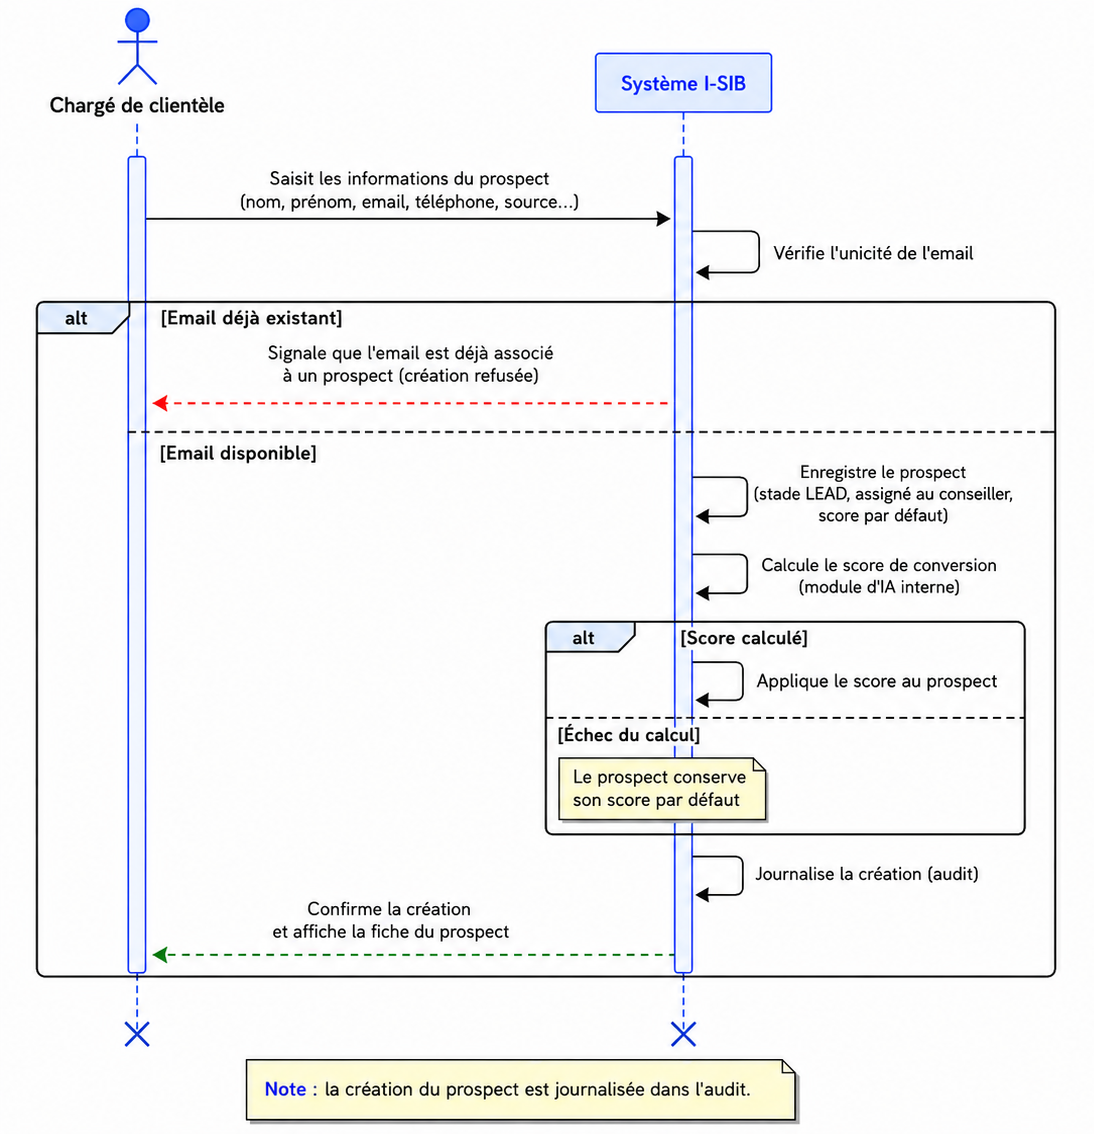
\includegraphics[width=\dimexpr\textwidth-2\fboxsep-2\fboxrule\relax]{images/contenu/chapitre-2/rc_seq_prospects.png}
    \caption{Mise à jour du pipeline et recalcul du score de conversion d'un prospect}
    \label{fig:rc_prospects}
\end{figure}

% ─────────────────────────────────────────────────
\subsection{Module SGI}

Le module SGI intègre les services d'investissement au sein de la plateforme I-SIB. Il
permet au client d'initier des opérations sur titres et offre aux équipes SGI les outils
nécessaires pour contrôler, valider et exécuter ces opérations. Dans le cadre de ce
chapitre, la fonctionnalité retenue pour ce module est le \textbf{passage d'ordres}, car
elle matérialise le lien opérationnel entre le client et la société de gestion et
d'intermédiation.

% ─────────────────────────────────────────────────
\subsubsection{Passage d'ordres}

Le passage d'ordres constitue le lien opérationnel entre le client et l'équipe SGI. Il
permet au client d'exprimer une intention d'achat ou de vente, et à l'équipe SGI de
contrôler, valider ou rejeter la demande selon les règles métier en vigueur. La
fiche~\ref{tab:sgi_ordres} en présente la description détaillée.

\begin{table}[H]
\centering
\caption{Fiche descriptive -- Passage d'ordres}
\label{tab:sgi_ordres}
\renewcommand{\arraystretch}{1.5}
\begin{tabular}{|>{\bfseries}p{3.8cm}|p{10.5cm}|}
\hline
Identifiant        & FSGI-01 \\ \hline
Acteurs            & Client, Équipe SGI \\ \hline
Préconditions      &
\begin{minipage}[t]{\linewidth}\vspace{2pt}
\begin{itemize}[leftmargin=*,topsep=0pt,itemsep=1pt,parsep=0pt]
    \item Le client est authentifié et son dossier KYC est complet
    \item Le titre visé est référencé et disponible sur la plateforme
    \item Le service de notification est opérationnel
\end{itemize}
\vspace{2pt}\end{minipage} \\ \hline
Scénario nominal   &
\begin{minipage}[t]{\linewidth}\vspace{2pt}
\begin{enumerate}[leftmargin=*,topsep=0pt,itemsep=2pt,parsep=0pt]
    \item Le client saisit un ordre en précisant le titre, le sens
          (achat ou vente) et la quantité souhaitée
    \item Le système enregistre l'ordre avec le statut \textit{Saisi}
          et notifie l'équipe SGI
    \item L'équipe SGI prend en charge l'ordre ; le statut passe à
          \textit{En cours de traitement} ; le client est notifié
    \item L'équipe SGI examine la demande et valide l'ordre ; le statut
          passe à \textit{Validé} ; le client est notifié de la validation
    \item L'ordre est exécuté sur le marché ; le statut passe à
          \textit{Exécuté} ; le portefeuille du client est mis à jour
    \item Le client reçoit une notification de confirmation d'exécution
\end{enumerate}
\vspace{2pt}\end{minipage} \\ \hline
Scénario alternatif &
\textbf{A1 -- Rejet de l'ordre :} si l'ordre ne respecte pas les règles métier
(quantité insuffisante, titre non autorisé, dossier KYC incomplet), l'équipe SGI
le rejette avec un motif explicite ; le statut passe à \textit{Rejeté} et le
client est notifié avec le motif communiqué \\ \hline
Scénario d'exception &
\textbf{E1 -- Échec technique lors de l'exécution :} le système ne peut finaliser
l'opération ; l'ordre est conservé au statut \textit{Validé} et une alerte est
envoyée à l'équipe SGI pour un retraitement manuel \\ \hline
Postconditions     & L'ordre est traité et archivé avec son statut final ;
                     le portefeuille du client est mis à jour en cas
                     d'exécution réussie \\ \hline
\end{tabular}
\end{table}

La figure~\ref{fig:sgi_ordres} représente le déroulement de cette fonctionnalité à
travers un diagramme de séquence.

\begin{figure}[H]
    \centering
    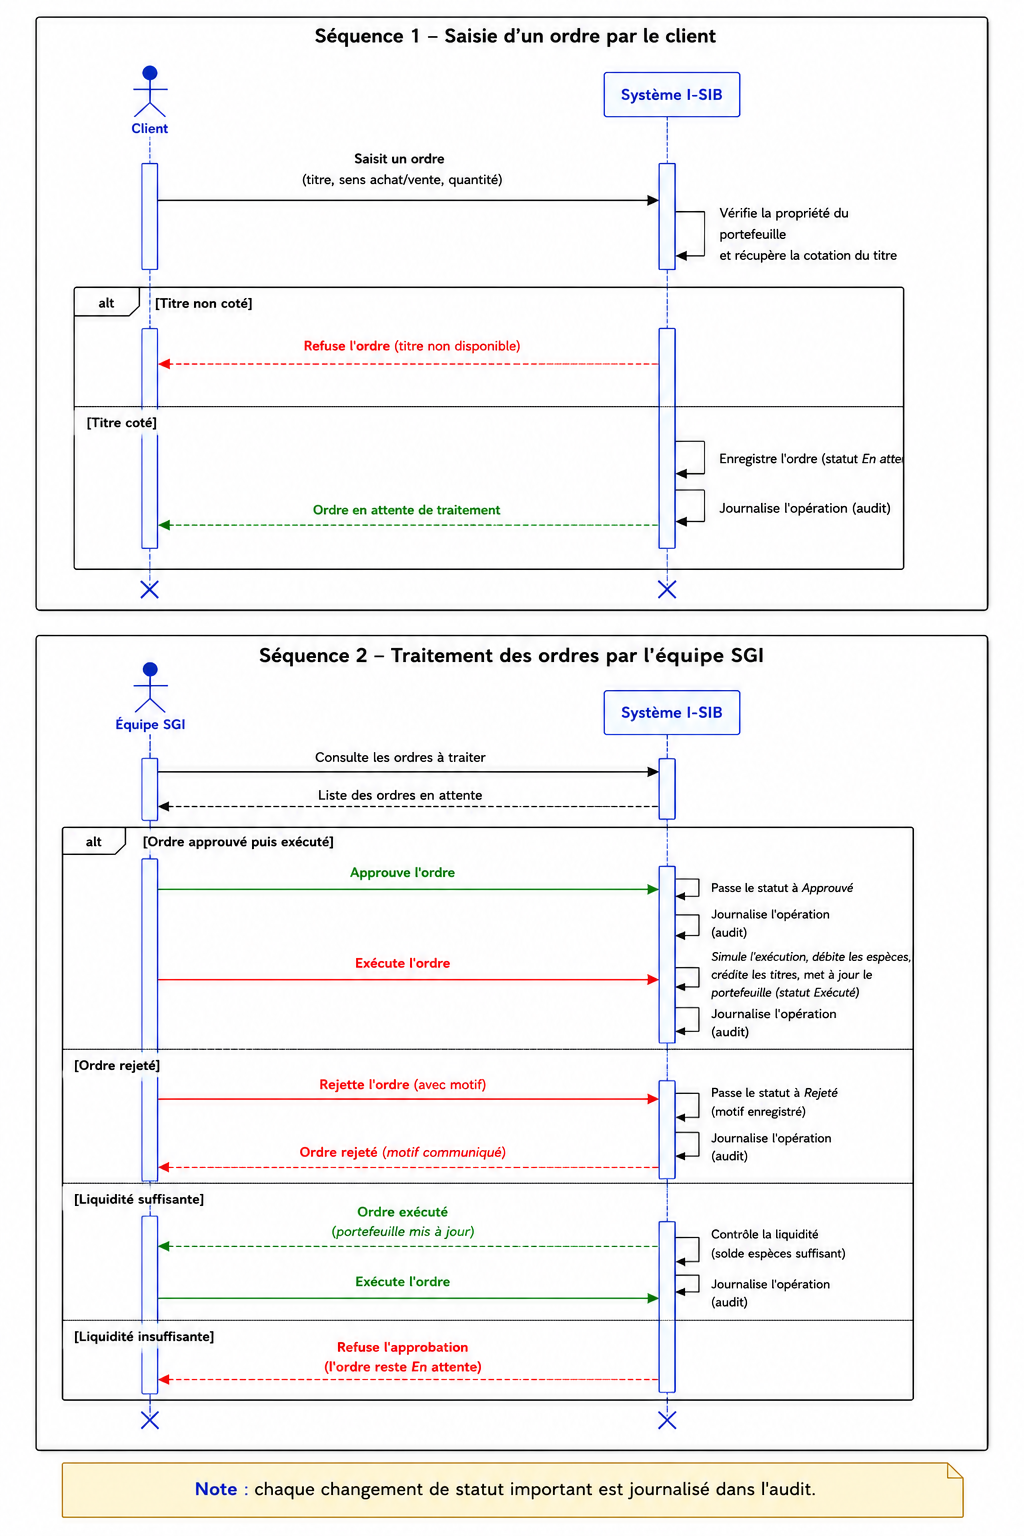
\includegraphics[width=\dimexpr\textwidth-2\fboxsep-2\fboxrule\relax]{images/contenu/chapitre-2/sgi_seq_passage_ordres.png}
    \caption{Circuit de soumission et de traitement d'un ordre de bourse du client à l'exécution}
    \label{fig:sgi_ordres}
\end{figure}
\newpage{}
% ─────────────────────────────────────────────────
\section{Exigences non fonctionnelles}

En plus des fonctionnalités, le système doit respecter plusieurs exigences non
fonctionnelles. Ces exigences déterminent la qualité globale de la solution et sont
particulièrement importantes dans un environnement bancaire. Elles encadrent la manière
dont le système doit être conçu, sécurisé, maintenu et utilisé. Elles s'inscrivent dans
les principes généraux de qualité logicielle \cite{iso25010}, de sécurité applicative
\cite{owasp_asvs} et de conformité des parcours d'identification client
\cite{fatf_digital_id}.

\begin{description}
    \item[Sécurité] Les accès doivent être contrôlés par rôle. Un client ne doit accéder
          qu'à ses propres données, tandis que les utilisateurs internes doivent disposer
          d'autorisations adaptées à leurs responsabilités.

    \item[Confidentialité] Les données personnelles, KYC, bancaires et d'investissement
          doivent être protégées contre tout accès non autorisé.

    \item[Traçabilité] Les actions importantes doivent être historisées : consultation
          sensible, modification de données, validation ou rejet d'ordre, et mise à jour
          de statut.

    \item[Disponibilité] Le système doit être accessible de manière continue afin de
          permettre la consultation des informations et le suivi des opérations.

    \item[Évolutivité] La solution doit pouvoir intégrer de nouvelles fonctionnalités et
          de nouveaux modules sans remettre en cause l'ensemble de l'architecture existante.

    \item[Ergonomie] Les interfaces doivent être simples, lisibles et adaptées aux profils
          utilisateurs afin de réduire les erreurs et de faciliter l'adoption du système.
\end{description}

La sécurité et la confidentialité sont prioritaires, car le système manipule des
informations sensibles. La traçabilité est indispensable pour reconstituer les opérations
et répondre aux exigences de contrôle. L'ergonomie doit être prise en compte dès la
conception, car un système complet mais difficile à utiliser risque d'être insuffisamment
adopté.

% ─────────────────────────────────────────────────
\section*{Conclusion}
\phantomsection
\addcontentsline{toc}{section}{Conclusion}

Ce chapitre a permis d'identifier les besoins fonctionnels et non fonctionnels du système
I-SIB pour les modules Relation Client et SGI. Les fonctionnalités retenues couvrent la
gestion des prospects pour le module Relation Client et le passage d'ordres pour le module
SGI. Chaque fonctionnalité a été détaillée à travers une fiche textuelle structurée et
illustrée par un diagramme de séquence. Ces besoins s'accompagnent
d'exigences essentielles en matière de sécurité, de confidentialité, de performance et de
traçabilité.

Cette analyse constitue la base de la conception fonctionnelle et technique du système,
présentée dans le chapitre suivant.

% ─────────────────────────────────────────────────
%  CHAPITRE 3 – CONCEPTION DE LA SOLUTION
% ─────────────────────────────────────────────────
\chapter{Conception de la solution}
\markboth{Conception de la solution}{Conception de la solution}

\section*{Introduction}
\phantomsection
\addcontentsline{toc}{section}{Introduction}

Ce chapitre traduit les besoins identifiés au chapitre précédent en une solution
structurée et implémentable. Il présente d'abord les principes retenus pour organiser
la plateforme, puis l'architecture fonctionnelle d'I-SIB, les choix technologiques,
l'architecture technique, la conception détaillée de la fonctionnalité Gestion des
prospects et enfin l'architecture de déploiement.

% ─────────────────────────────────────────────────
\section{Principes de conception de l'architecture}

En prenant en compte les besoins fonctionnels et non fonctionnels identifiés au chapitre
précédent, la conception de la solution doit s'appuyer sur des principes d'organisation
clairs. Ces principes permettent d'orienter les choix d'architecture afin de répondre aux
contraintes du contexte bancaire, notamment la sécurité des accès, la protection des
données, la traçabilité des opérations et l'évolution progressive des modules métier.
Cette section présente donc les principes retenus, qui serviront de base à l'architecture
globale de la plateforme, en cohérence avec les principes de qualité logicielle
\cite{iso25010} et de sécurité applicative \cite{owasp_asvs}.

Les principaux principes retenus sont les suivants :

\begin{itemize}
    \item \textbf{Séparer les responsabilités} afin que chaque module conserve un périmètre
          clair, notamment pour la Relation Client, la SGI, l'authentification, l'audit et
          les services transversaux.
    \item \textbf{Centraliser les accès} pour éviter que les applications clientes ne
          communiquent directement avec les services internes.
    \item \textbf{Protéger les données sensibles} en limitant les accès selon les rôles et
          en isolant les informations manipulées par les différents services.
    \item \textbf{Assurer la traçabilité} des opérations importantes, en particulier les
          actions liées au KYC, aux prospects, aux portefeuilles et aux ordres de bourse.
    \item \textbf{Faciliter l'évolution du système} afin de pouvoir ajouter de nouveaux
          modules ou de nouvelles fonctionnalités sans remettre en cause toute la
          plateforme.
    \item \textbf{Maintenir une expérience utilisateur cohérente} entre les interfaces
          destinées aux clients et celles utilisées par les équipes internes.
\end{itemize}

Ces principes conduisent à retenir une architecture modulaire, organisée autour de blocs
spécialisés qui communiquent entre eux de manière contrôlée \cite{fowler_microservices}.
\newpage{}
% ─────────────────────────────────────────────────
\section{Architecture fonctionnelle de la solution}

\subsection{Vue d'ensemble}

La solution I-SIB repose sur une architecture microservices organisée en plusieurs couches. Les utilisateurs accèdent à la plateforme via deux interfaces web : un back-office pour les employés et un front-office pour les clients. Les requêtes passent par une passerelle API chargée de l’authentification et du routage vers les microservices concernés.

L’architecture regroupe les interfaces utilisateur, les services métier ainsi que les composants techniques assurant la sécurité, le routage, le stockage des données, le cache, la messagerie et la traçabilité. La figure~\ref{fig:architecture_fonctionnelle} présente l’organisation fonctionnelle de ces composants et leurs interactions.



\begin{figure}[H]
    \centering
    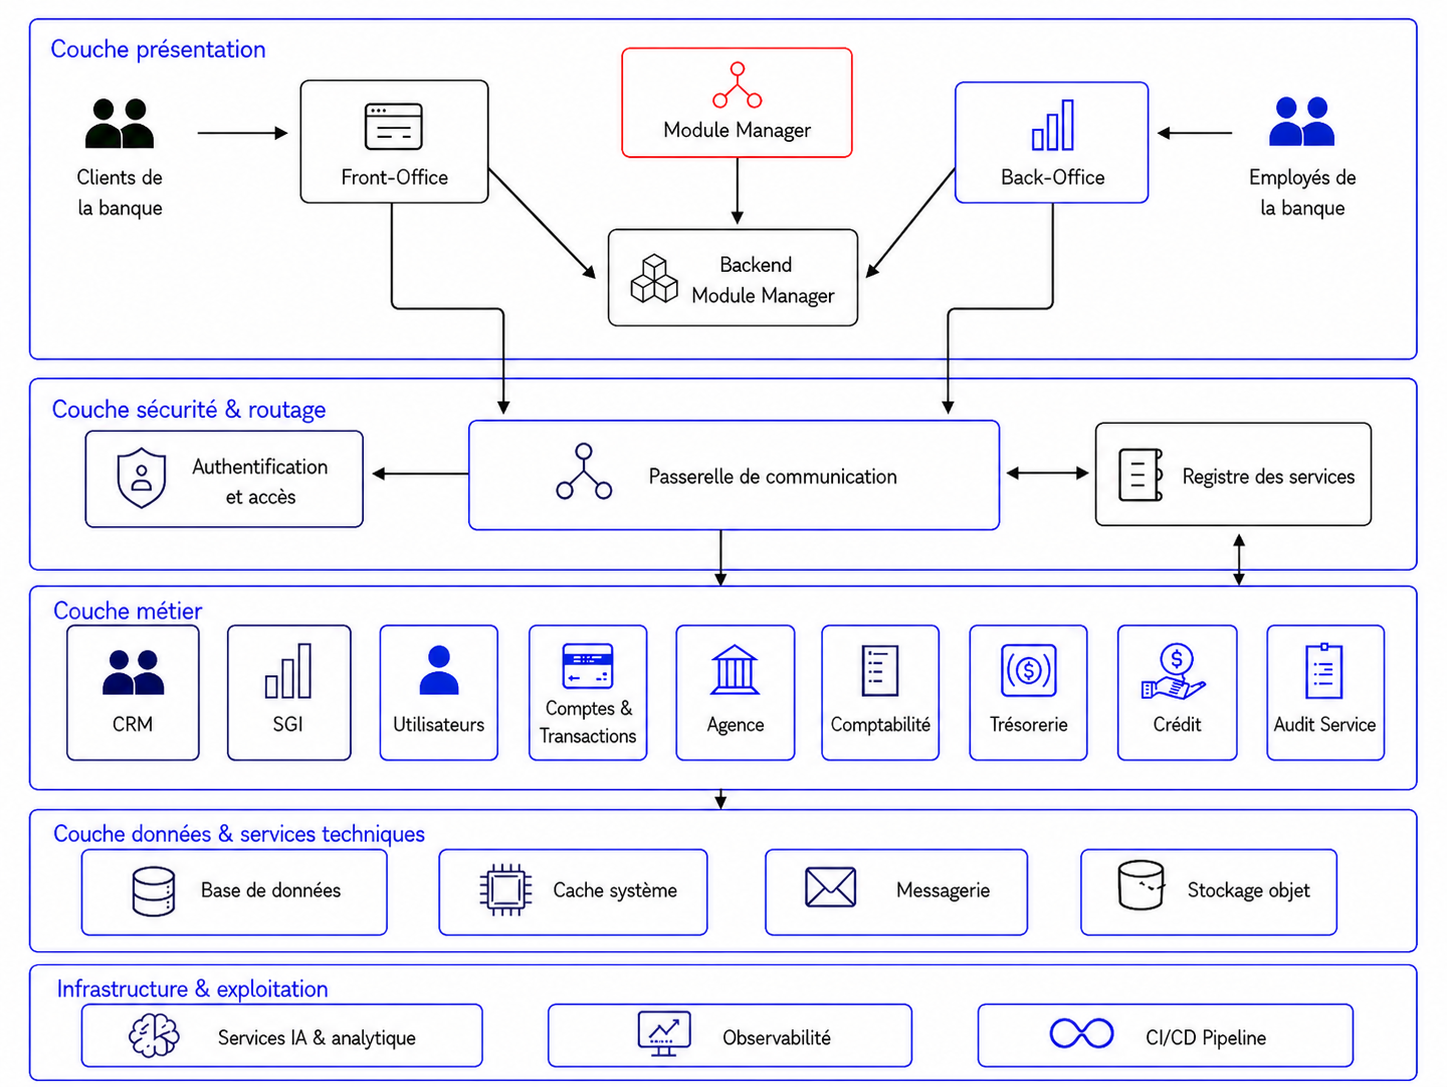
\includegraphics[width=\dimexpr\textwidth-2\fboxsep-2\fboxrule\relax]{images/contenu/chapitre-3/architecture_fonctionnelle.png}
    \caption{Architecture fonctionnelle de la plateforme I-SIB}
    \label{fig:architecture_fonctionnelle}
\end{figure}

Comme le montre la figure~\ref{fig:architecture_fonctionnelle}, la passerelle API joue
un rôle central : elle constitue la frontière entre les applications web et les
microservices internes. Les services métier restent ainsi isolés de tout accès
direct depuis l'extérieur.
\newpage{}
\subsection{Description des blocs}

La figure~\ref{fig:architecture_fonctionnelle} est organisée autour de plusieurs blocs
complémentaires, chacun correspondant à une responsabilité précise dans la plateforme.

\begin{description}
    \item[Front-office] Espace destiné aux clients de la banque. Il permet de consulter
          les comptes, les transactions, les portefeuilles et les ordres de bourse depuis
          une interface en libre-service.

    \item[Back-office] Espace réservé aux employés. Il regroupe les modules utilisés par
          les chargés de clientèle, les gestionnaires SGI, les équipes d'agence, la
          trésorerie, la comptabilité et l'administration.

    \item[Authentification et accès] Bloc chargé de contrôler l'identité des utilisateurs,
          les rôles, les sessions et les règles de sécurité avant l'accès aux services.

    \item[Passerelle de communication] Point d'entrée central entre les interfaces et les
          microservices. Elle sécurise les échanges, valide les requêtes, applique les
          contrôles d'accès et route les demandes vers les services concernés.

    \item[Registre des services] Annuaire permettant de localiser les services actifs et
          de suivre leur état. Il facilite la communication entre la passerelle et les
          microservices internes.

    \item[Services métier] Ensemble des microservices qui portent les fonctionnalités de
          la plateforme : Relation Client, SGI, utilisateurs, comptes et transactions,
          agence, comptabilité, trésorerie et crédit.

    \item[Audit service] Bloc dédié à la journalisation des événements, à l'historique des
          actions sensibles et au suivi de la conformité réglementaire.

    \item[Données et services de support] Ensemble des composants de support aux
          traitements métier : base de données, cache système, messagerie asynchrone et
          stockage objet des fichiers et documents.

    \item[Services IA et analytique] Bloc qui regroupe l'assistant intelligent, l'analyse
          prédictive et la segmentation client afin d'apporter une aide à la décision.

    \item[Observabilité et déploiement] Ensemble des éléments qui facilitent l'exploitation
          de la plateforme : logs, traçabilité des requêtes, intégration continue,
          déploiement automatisé et orchestration des conteneurs.
\end{description}
\newpage{}
\section{Choix des outils et technologies}

Les choix technologiques traduisent l'architecture fonctionnelle en composants
réalisables. Ils ont été retenus en fonction des responsabilités à couvrir :
interfaces web, services backend, sécurité, routage, persistance des données,
messagerie, cache, stockage documentaire, traçabilité et déploiement. Cette section
présente les principaux outils utilisés et précise le rôle de chacun dans la plateforme
I-SIB. La section suivante montrera comment ces technologies s'assemblent concrètement
dans l'architecture technique de la solution.

Les interfaces web de la plateforme sont développées avec \textbf{Next.js 16}
\cite{nextjs_docs} et \textbf{TypeScript} \cite{typescript_docs}, afin de construire des applications front-office et back-office
modernes, maintenables et adaptées aux différents profils utilisateurs. Le backend repose
sur \textbf{Spring Boot 3.5} \cite{spring_boot_docs}, utilisé comme socle de développement des microservices
métier. L'accès aux services est centralisé par \textbf{Spring Cloud Gateway}
\cite{spring_gateway_docs}, qui assure
le routage, les filtres de sécurité et la résilience. La gestion des identités et des
rôles est confiée à \textbf{Keycloak} \cite{keycloak_docs}, tandis que
\textbf{Netflix Eureka} \cite{spring_eureka_docs} permet la découverte dynamique des services.

Pour la persistance, \textbf{PostgreSQL} est retenu comme système de gestion de bases de
données relationnel \cite{postgresql_docs}, avec une base isolée par microservice afin de préserver l'autonomie
des données. \textbf{Redis} \cite{redis_docs} est utilisé pour le cache et le contrôle de débit, tandis que
\textbf{RabbitMQ} \cite{rabbitmq_docs} prend en charge la communication asynchrone entre les services,
notamment pour les événements d'audit. Les documents clients et les pièces KYC sont
stockés dans \textbf{MinIO} \cite{minio_docs}, qui permet de gérer un stockage objet sécurisé.

Les fonctionnalités d'intelligence artificielle s'appuient notamment sur \textbf{Rasa}
\cite{rasa_docs}
pour le chatbot conversationnel et sur des services spécialisés de scoring ou de
segmentation. La traçabilité technique est assurée par \textbf{Zipkin} \cite{zipkin_docs}, qui permet de
suivre les appels entre microservices. Enfin, \textbf{Docker} \cite{docker_docs} et
\textbf{Docker Compose} \cite{docker_compose_docs}
facilitent la conteneurisation, l'organisation des composants et leur déploiement dans des
stacks séparées.

\section{Architecture technique de la solution}

Après le choix des outils, l'architecture technique précise la manière dont ces
technologies sont assemblées pour faire fonctionner la plateforme. Elle met en relation
les applications web, la passerelle API, les microservices, les bases de données et les
composants transversaux nécessaires à la sécurité, à la communication et à
l'observabilité.

Dans cette architecture, les applications front-office et back-office consomment les API
exposées par la passerelle. Celle-ci constitue le point d'entrée technique vers les
services internes et applique les règles de sécurité et de routage. Les microservices
métier, dont le service Relation Client et le service SGI, disposent chacun de leur propre
persistance et communiquent avec les services transversaux selon les besoins de leurs
traitements.

Cette organisation permet de matérialiser les principes définis précédemment tout en
préparant le passage vers la conception détaillée des fonctionnalités. La
figure~\ref{fig:architecture_technique} montre les liens entre les technologies retenues
et les composants applicatifs.

\begin{figure}[H]
    \centering
    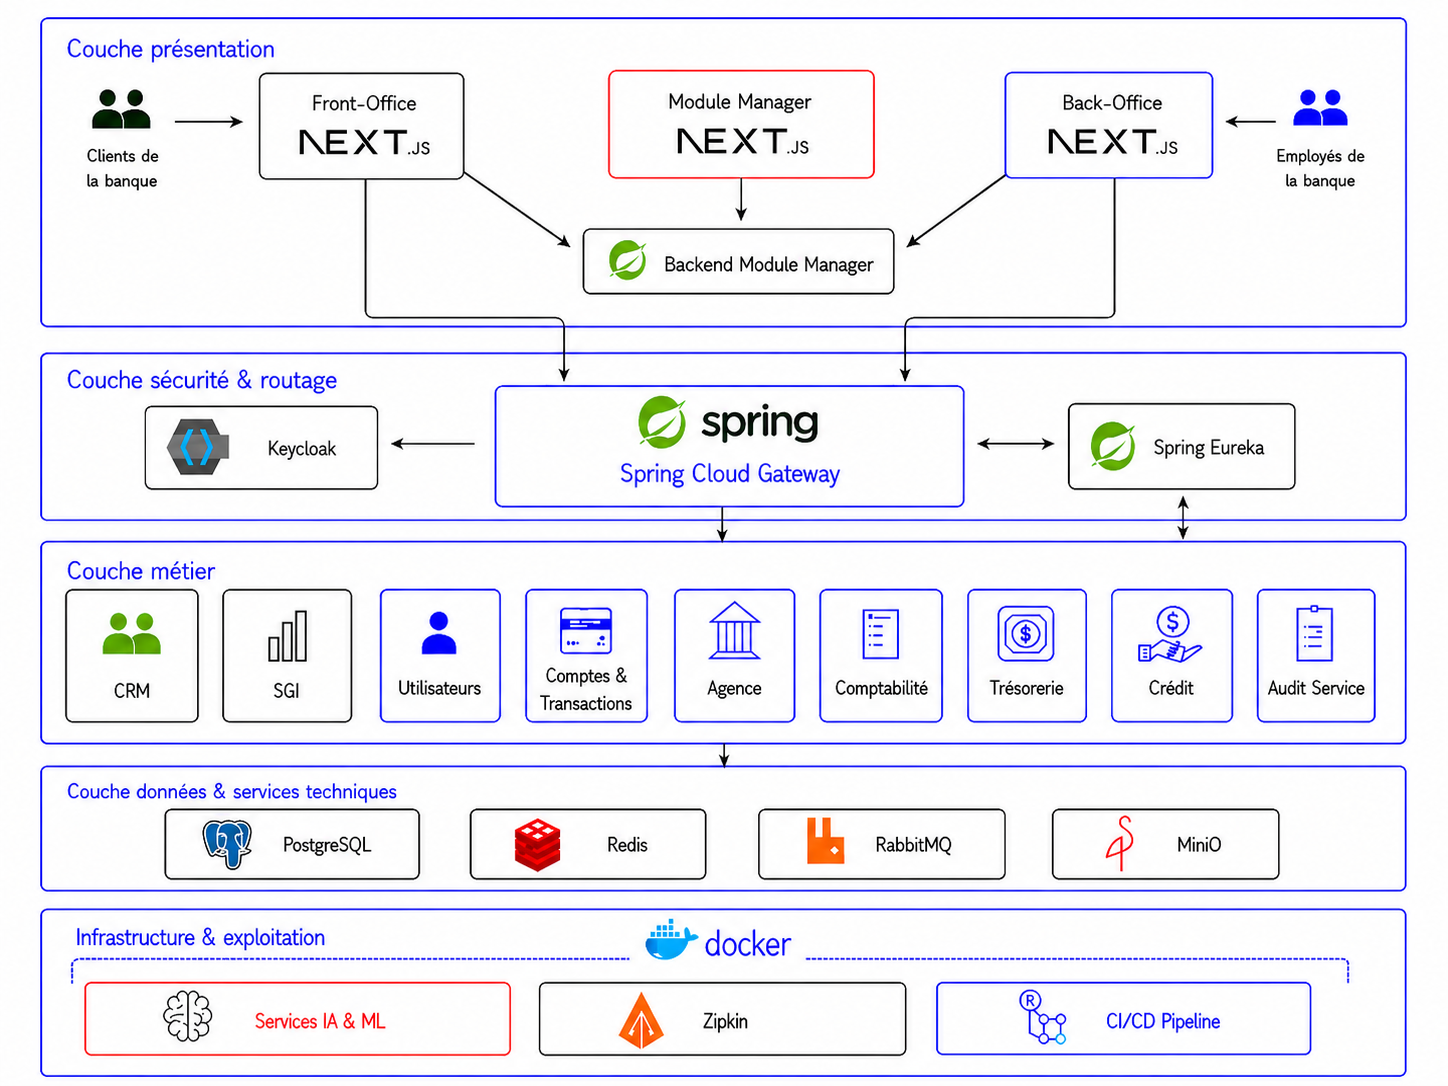
\includegraphics[width=\dimexpr\textwidth-2\fboxsep-2\fboxrule\relax]{images/contenu/chapitre-3/architecture_technique.png}
    \caption{Architecture technique de la plateforme I-SIB}
    \label{fig:architecture_technique}
\end{figure}

% ─────────────────────────────────────────────────
\section{Conception détaillée}

Après la présentation des architectures fonctionnelle et technique, cette section détaille
le fonctionnement interne d'une fonctionnalité représentative du module Relation Client :
la \textbf{Gestion des prospects}. Ce choix permet d'illustrer, de manière ciblée, le
cheminement d'une demande depuis l'interface back-office jusqu'aux services backend, en
passant par la passerelle API, le service CRM, la base de données, le scoring par
intelligence artificielle et la traçabilité.

La section présente successivement le périmètre de la fonctionnalité retenue, le workflow
de traitement illustré par deux figures portant sur la création d'un prospect et sa
conversion en client, une synthèse des principales API exposées sous forme de tableau,
puis une vue de conception montrant les artefacts mobilisés et leurs relations.

\subsection{Périmètre de la fonctionnalité}

La gestion des prospects couvre le suivi d'un contact commercial depuis son
enregistrement jusqu'à sa qualification, sa conversion en client ou son abandon. L'acteur
principal est le chargé de clientèle, qui consulte les prospects qui lui sont affectés,
met à jour leur étape dans le pipeline, ajoute des interactions et planifie les relances.
Le service CRM assure le traitement métier, tandis que les services transversaux
interviennent pour le scoring, la persistance et l'audit.

\subsection{Workflow de traitement}

Le workflow de la gestion des prospects est présenté à travers deux opérations
représentatives : la création d'un prospect et sa conversion en client. Ces deux cas
permettent de montrer le cheminement d'une demande depuis le back-office jusqu'aux
services backend, ainsi que l'intervention des services de scoring, de persistance et
d'audit.

La création d'un prospect commence par la saisie des informations dans la vue Prospects.
La demande est transmise à la passerelle API, puis routée vers le service CRM. Celui-ci
contrôle les informations reçues, persiste le prospect, sollicite le service de scoring IA
et publie une trace d'audit. La figure~\ref{fig:workflow_creation_prospect} illustre ce
premier scénario.

\begin{figure}[H]
    \centering
    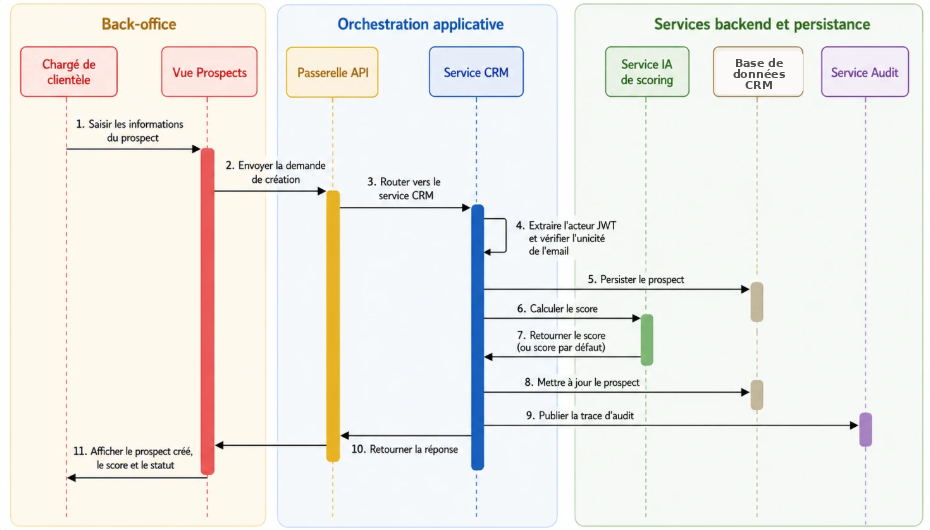
\includegraphics[width=\dimexpr\textwidth-2\fboxsep-2\fboxrule\relax]{images/contenu/chapitre-3/workflow_creation_prospect.png}
    \caption{Workflow de création d'un prospect avec scoring IA}
    \label{fig:workflow_creation_prospect}
\end{figure}

La conversion d'un prospect intervient lorsqu'un prospect qualifié doit devenir client.
Le service CRM vérifie l'éligibilité du prospect, sollicite le service de segmentation,
crée le compte client, initialise le scoring associé, déclenche l'envoi du courriel de
bienvenue et historise l'opération. La figure~\ref{fig:workflow_conversion_prospect}
présente ce second scénario.

\begin{figure}[H]
    \centering
    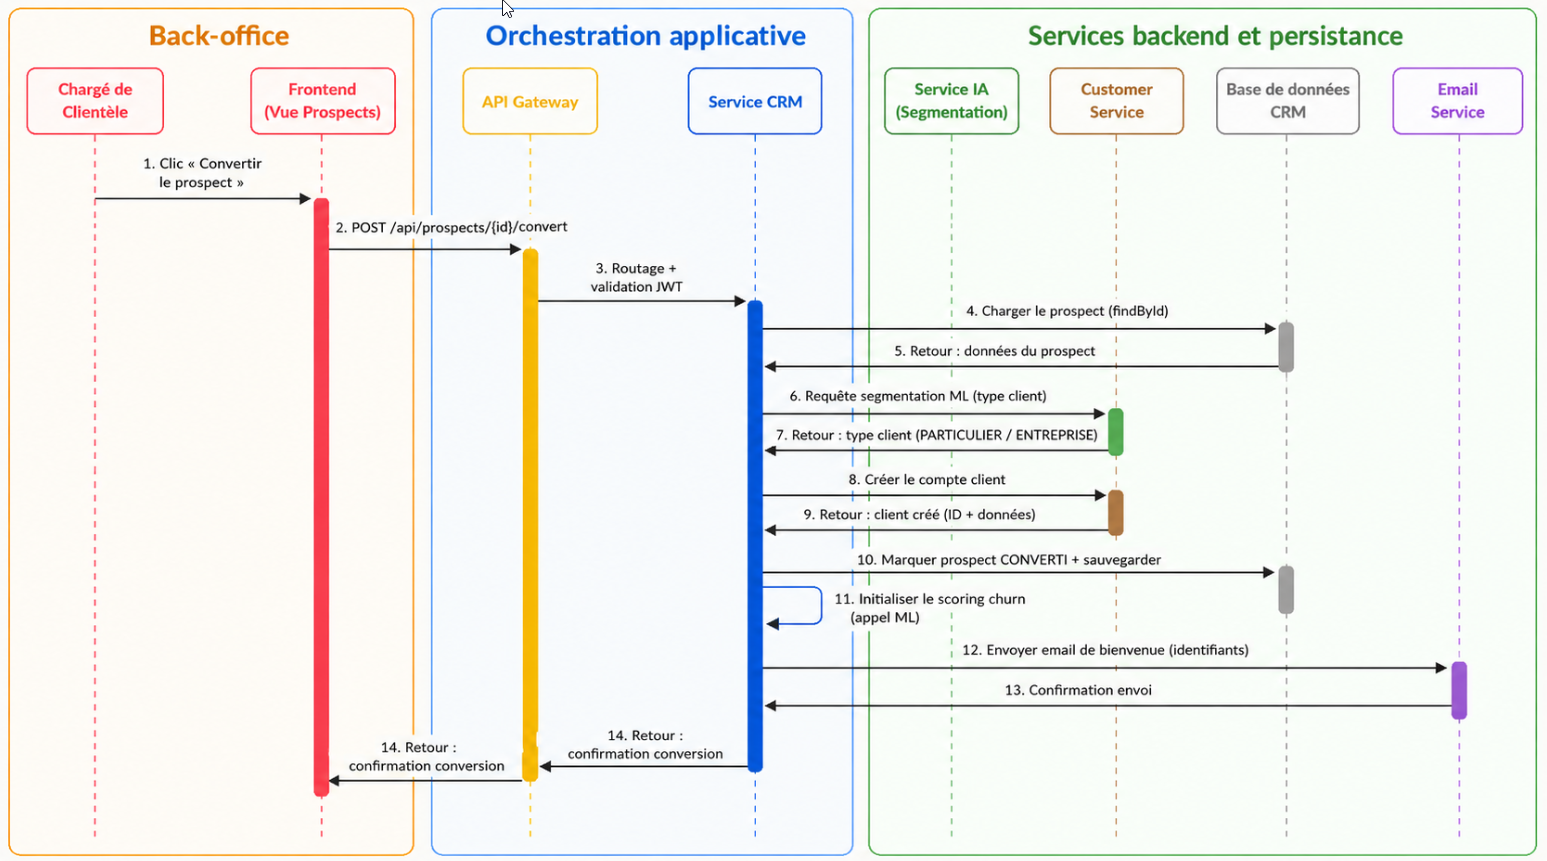
\includegraphics[width=\dimexpr\textwidth-2\fboxsep-2\fboxrule\relax]{images/contenu/chapitre-3/workflow_conversion_prospect.png}
    \caption{Workflow de conversion d'un prospect en client}
    \label{fig:workflow_conversion_prospect}
\end{figure}

\subsection{Synthèse des API}

Les opérations de la fonctionnalité sont exposées sous forme d'API REST sécurisées. Le
tableau~\ref{tab:endpoints_prospect} présente une synthèse volontairement limitée aux
endpoints les plus représentatifs.

\begin{table}[H]
\centering
\caption{Synthèse des principales API de gestion des prospects}
\label{tab:endpoints_prospect}
\small
\renewcommand{\arraystretch}{1.3}
\begin{tabular}{|p{1.7cm}|p{6.0cm}|p{5.5cm}|}
\hline
\textbf{Méthode} & \textbf{Chemin} & \textbf{Utilisation principale} \\ \hline
POST   & \texttt{/api/crm/prospects}                  & Enregistrer un nouveau prospect \\ \hline
GET    & \texttt{/api/crm/prospects/}\newline\texttt{my-prospects}     & Afficher les prospects du chargé connecté \\ \hline
GET    & \texttt{/api/crm/prospects/\{id\}}           & Consulter la fiche détaillée d'un prospect \\ \hline
PATCH  & \texttt{/api/crm/prospects/\{id\}}           & Mettre à jour les informations ou l'étape \\ \hline
POST   & \texttt{/api/crm/prospects/\{id\}/}\newline\texttt{activities} & Ajouter une interaction ou une relance \\ \hline
POST   & \texttt{/api/crm/prospects/\{id\}/}\newline\texttt{convert}   & Transformer un prospect qualifié en client \\ \hline
\end{tabular}
\end{table}

\subsection{Vue de conception de la fonctionnalité}

La vue de conception complète le workflow en montrant les artefacts applicatifs impliqués
dans la fonctionnalité. Elle reprend les stéréotypes de Jacobson : les éléments
\textit{boundary} représentent les interfaces, les éléments \textit{control} portent la
coordination applicative, et les éléments \textit{entity} correspondent aux données métier
manipulées par le système \cite{jacobson_oose}.

La figure~\ref{fig:conception_gestion_prospects} présente cette vue de conception en
mettant en relation les interfaces, les composants de contrôle et les entités métier de
la fonctionnalité Gestion des prospects.

\begin{figure}[H]
    \centering
    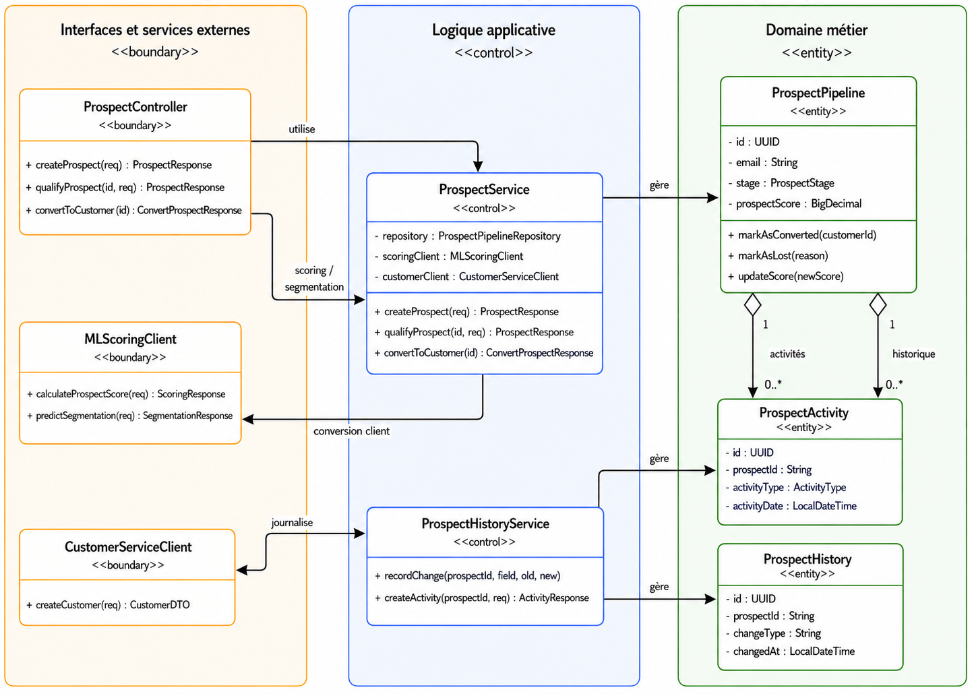
\includegraphics[width=\dimexpr\textwidth-2\fboxsep-2\fboxrule\relax]{images/contenu/chapitre-3/conception_gestion_prospects.png}
    \caption{Vue de conception de la fonctionnalité Gestion des prospects}
    \label{fig:conception_gestion_prospects}
\end{figure}

Ainsi, la conception détaillée de la gestion des prospects montre comment une
fonctionnalité métier s'appuie sur les couches définies précédemment : interface,
passerelle, service métier, données, intelligence artificielle et audit.

% ─────────────────────────────────────────────────
\section{Architecture de déploiement}

La vue logique de l'architecture est complétée par l'architecture mise en place
dans l'environnement de validation. La plateforme actuellement réalisée est
déployée sur un VPS AlmaLinux afin de tester progressivement les services
disponibles à mesure que le périmètre fonctionnel évolue. Cette seconde lecture
présente l'organisation des composants et la séparation des réseaux Docker.

Dans cet environnement de test, la plateforme I-SIB est décomposée en quatre
ensembles Docker Compose indépendants. Cette organisation suit une logique de
séparation des responsabilités au niveau infrastructurel : chaque ensemble peut
être redémarré, mis à jour ou répliqué sans impacter les autres. Les ensembles
\texttt{infra}, \texttt{core},
\texttt{module} et \texttt{office} distinguent respectivement les services
communs, les référentiels de base, les modules métier avancés et les interfaces
utilisateur \cite{docker_compose_docs}.

Deux réseaux Docker structurent la communication entre les conteneurs. Le réseau
\texttt{sib\_public} est réservé aux services accessibles depuis l'extérieur :
la passerelle API et les trois applications web. Le réseau \texttt{sib\_internal}
regroupe l'ensemble des microservices et des bases de données, totalement isolés
de tout accès direct depuis l'extérieur. Seule la passerelle appartient aux deux
réseaux simultanément, faisant office de frontière de sécurité.

La figure~\ref{fig:architecture_deploiement} reprend cette organisation sous forme
de schéma. Elle met en évidence la séparation entre les services exposés, les
services internes et le rôle particulier de la passerelle API entre les deux
réseaux.

\begin{figure}[H]
    \centering
    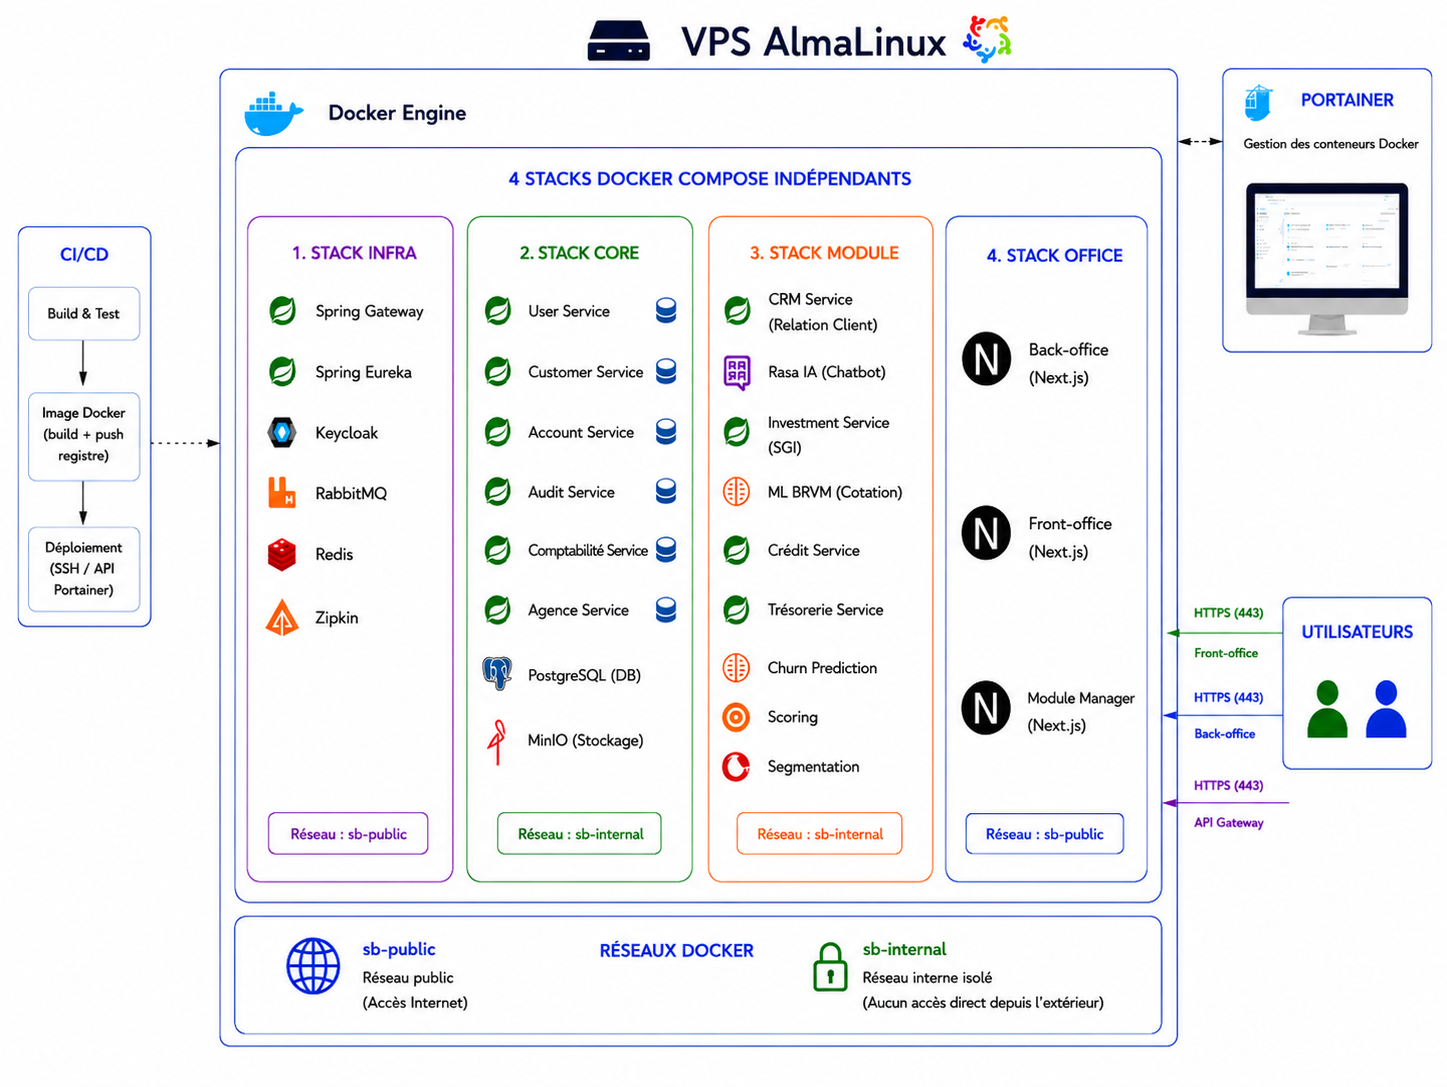
\includegraphics[width=\dimexpr\textwidth-2\fboxsep-2\fboxrule\relax]{images/contenu/chapitre-3/architecture_deploiement.png}
    \caption{Déploiement de validation d'I-SIB sur un VPS AlmaLinux}
    \label{fig:architecture_deploiement}
\end{figure}

Cette organisation prévoit un ordre de démarrage précis. L'ensemble \texttt{infra}
doit être lancé en premier afin de rendre disponibles la passerelle, Eureka,
Keycloak, Redis et RabbitMQ. L'ensemble \texttt{core} peut ensuite démarrer les
services de base. L'ensemble \texttt{module} vient après, car il dépend des
référentiels et de l'infrastructure. Enfin, l'ensemble \texttt{office} est lancé
en dernier pour exposer les interfaces utilisateur. À chaque évolution validée,
la chaîne de livraison permet de reconstruire et de redéployer les composants
concernés sur le VPS. Ce déploiement sert à la validation progressive de la
solution ; il ne constitue pas encore un environnement de production. Les
captures techniques permettant de documenter cette validation sont prévues en
annexe~\ref{ann:validation-deploiement}.
% ─────────────────────────────────────────────────
\section*{Conclusion}
\phantomsection
\addcontentsline{toc}{section}{Conclusion}

Ce chapitre a présenté la conception de la solution I-SIB pour les modules
Relation Client et SGI. L'architecture microservices retenue vise à répondre aux
exigences non fonctionnelles identifiées au chapitre précédent : la passerelle
et Keycloak soutiennent le contrôle des accès, Redis et l'indexation facilitent
la réactivité, RabbitMQ contribue à la traçabilité et Docker rend le déploiement
reproductible. Le déploiement de validation sur VPS AlmaLinux fournit un cadre
concret de vérification progressive. Le chapitre suivant présente les résultats
fonctionnels obtenus et les limites restant à traiter avant une mise en production.

% ─────────────────────────────────────────────────
%  CHAPITRE 4 – PRESENTATION DES RESULTATS ET ANALYSE CRITIQUE
% ─────────────────────────────────────────────────
\chapter{Présentation des résultats et analyse critique}
\markboth{Présentation des résultats et analyse critique}{Présentation des résultats et analyse critique}

\section*{Introduction}
\phantomsection
\addcontentsline{toc}{section}{Introduction}

Ce chapitre présente les résultats concrets obtenus à l'issue de la phase de
réalisation. Son objectif n'est pas de reprendre la conception technique déjà
présentée au chapitre précédent, mais de montrer comment les besoins exprimés
ont été concrétisés dans l'application \textbf{I-SIB}. La lecture proposée est
donc principalement fonctionnelle : elle met en relation les objectifs du projet,
les interfaces livrées et les usages qu'elles permettent.

Le chapitre est organisé en quatre parties. La première présente les résultats
obtenus pour le module \textbf{Relation Client} ; les interfaces y sont utilisées
comme supports d'illustration afin de montrer comment les fonctionnalités se
traduisent dans l'application. La deuxième adopte la même logique pour le module
\textbf{SGI}, à travers le pilotage des portefeuilles, la consultation des
cotations, l'analyse des palmarès de titres et le suivi des investissements. La
troisième propose une synthèse de la couverture des objectifs spécifiques sous
forme de tableau. Enfin, la dernière partie porte un regard critique sur la
réalisation, en distinguant les points forts, les limites actuelles et les
perspectives d'amélioration.

% ─────────────────────────────────────────────────
\section{Résultats côté Relation Client}

Le module \textbf{Relation Client} regroupe l'ensemble des fonctionnalités
permettant de connaître, suivre et fidéliser les clients de la banque. La
présentation ne consiste donc pas à commenter uniquement des captures d'écran ;
elle décrit d'abord les fonctionnalités réalisées, puis utilise les interfaces
comme preuves visuelles de leur mise en œuvre. Quatre fonctionnalités sont
retenues pour structurer cette partie : le portefeuille clients, la gestion des
comptes, l'agent IA de relation client et la gestion des prospects.

\subsection{Portefeuille clients}

La fonctionnalité de portefeuille clients centralise la connaissance client et
offre au chargé de clientèle une vue de travail unique. Elle regroupe des
indicateurs synthétiques, la liste détaillée des clients, leur statut, leur
niveau de risque, leurs comptes, leurs produits et le risque de départ estimé
par le modèle d'IA. Les filtres et la recherche facilitent l'accès rapide à un
client précis.

Cet écran matérialise deux objectifs : le \textbf{tableau de bord Relation
Client} adapté au chargé de clientèle et la \textbf{vue 360° client} sous sa
forme synthétique. La figure~\ref{fig:portefeuille_clients} présente cette vue
de portefeuille, qui sert de point d'entrée au suivi commercial.

\begin{figure}[H]
    \centering
    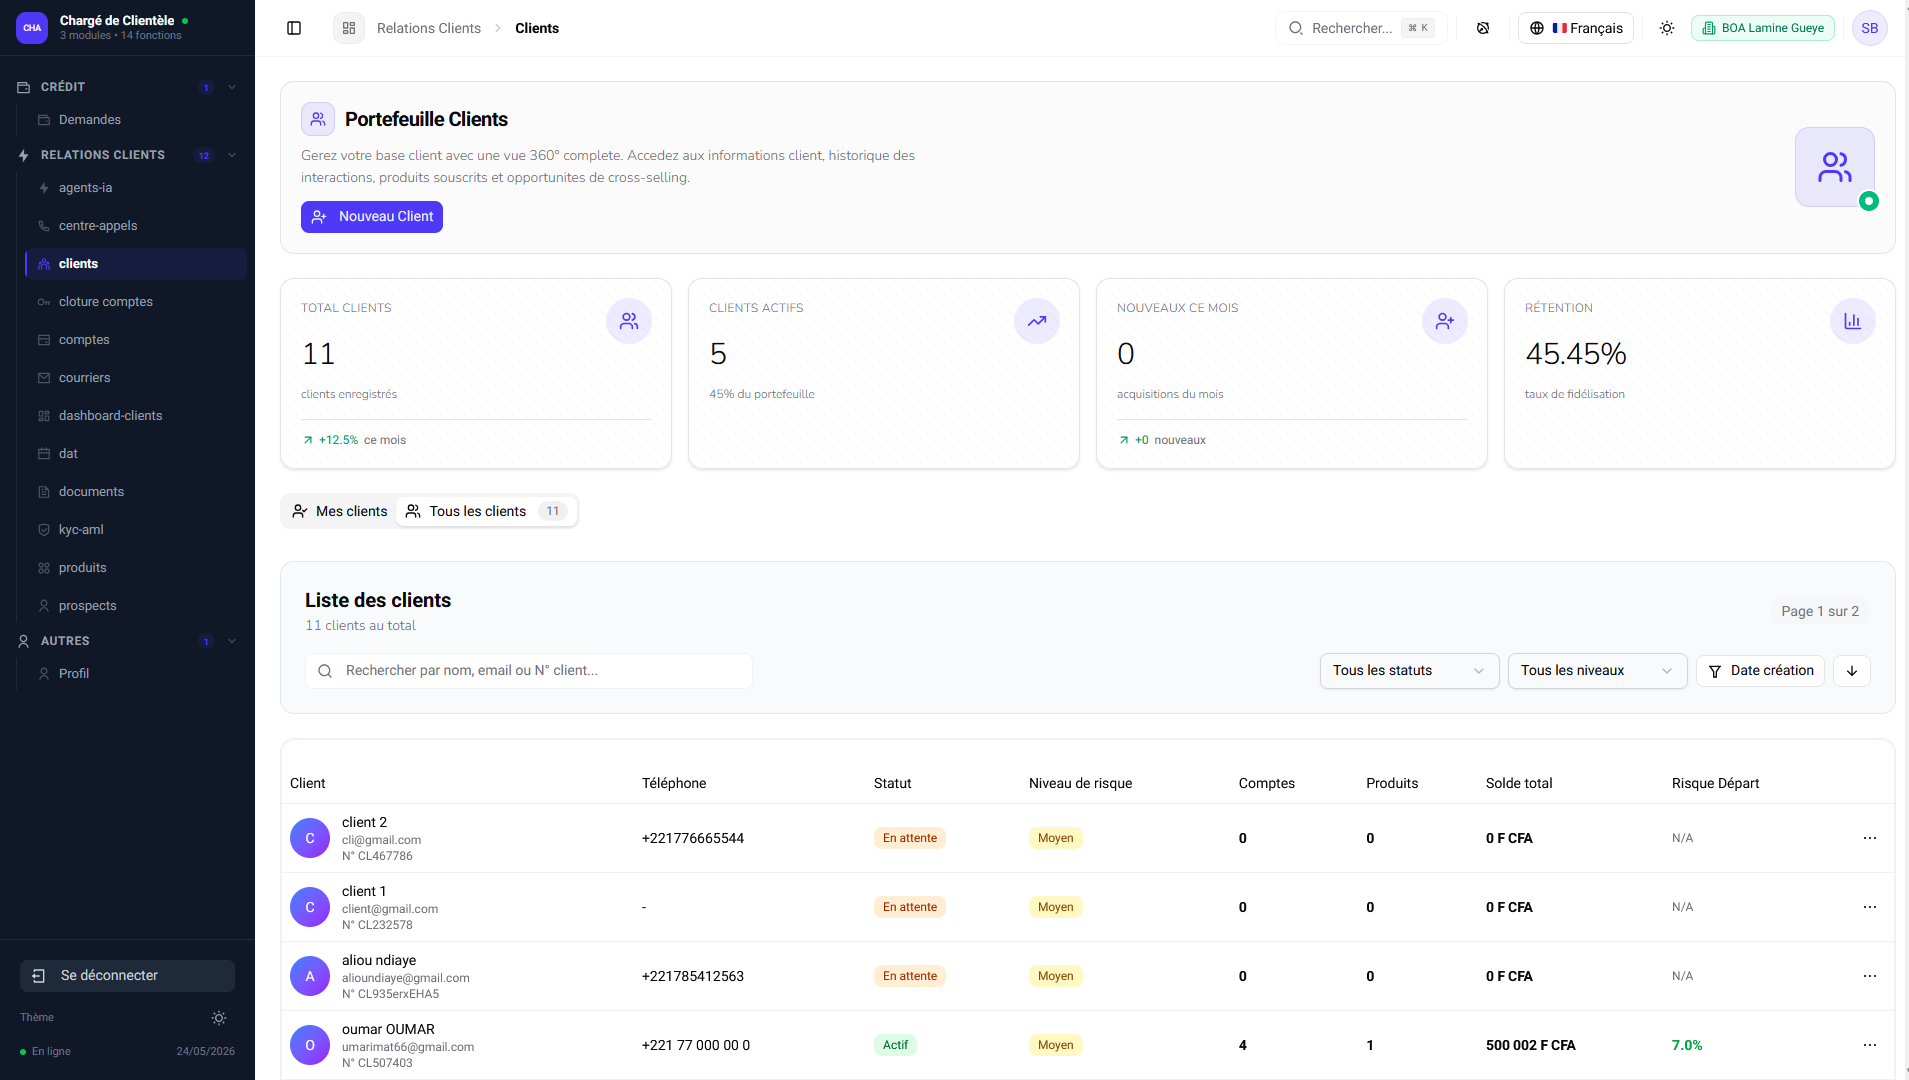
\includegraphics[width=0.88\textwidth]{images/contenu/chapitre-4/portefeuille_clients.png}
    \caption{Interface Portefeuille Clients du chargé de clientèle}
    \label{fig:portefeuille_clients}
\end{figure}

\subsection{Gestion des comptes}

La gestion des comptes complète la connaissance client en donnant accès aux
comptes bancaires associés à un client sélectionné. Pour chaque compte, le
système présente les informations principales : type de compte, numéro, IBAN,
solde et statut. La possibilité de télécharger les RIB illustre également la
\textbf{dématérialisation des documents} dans le parcours Relation Client.
La figure~\ref{fig:gestion_comptes} illustre cette consultation centralisée des
comptes bancaires.

\begin{figure}[H]
    \centering
    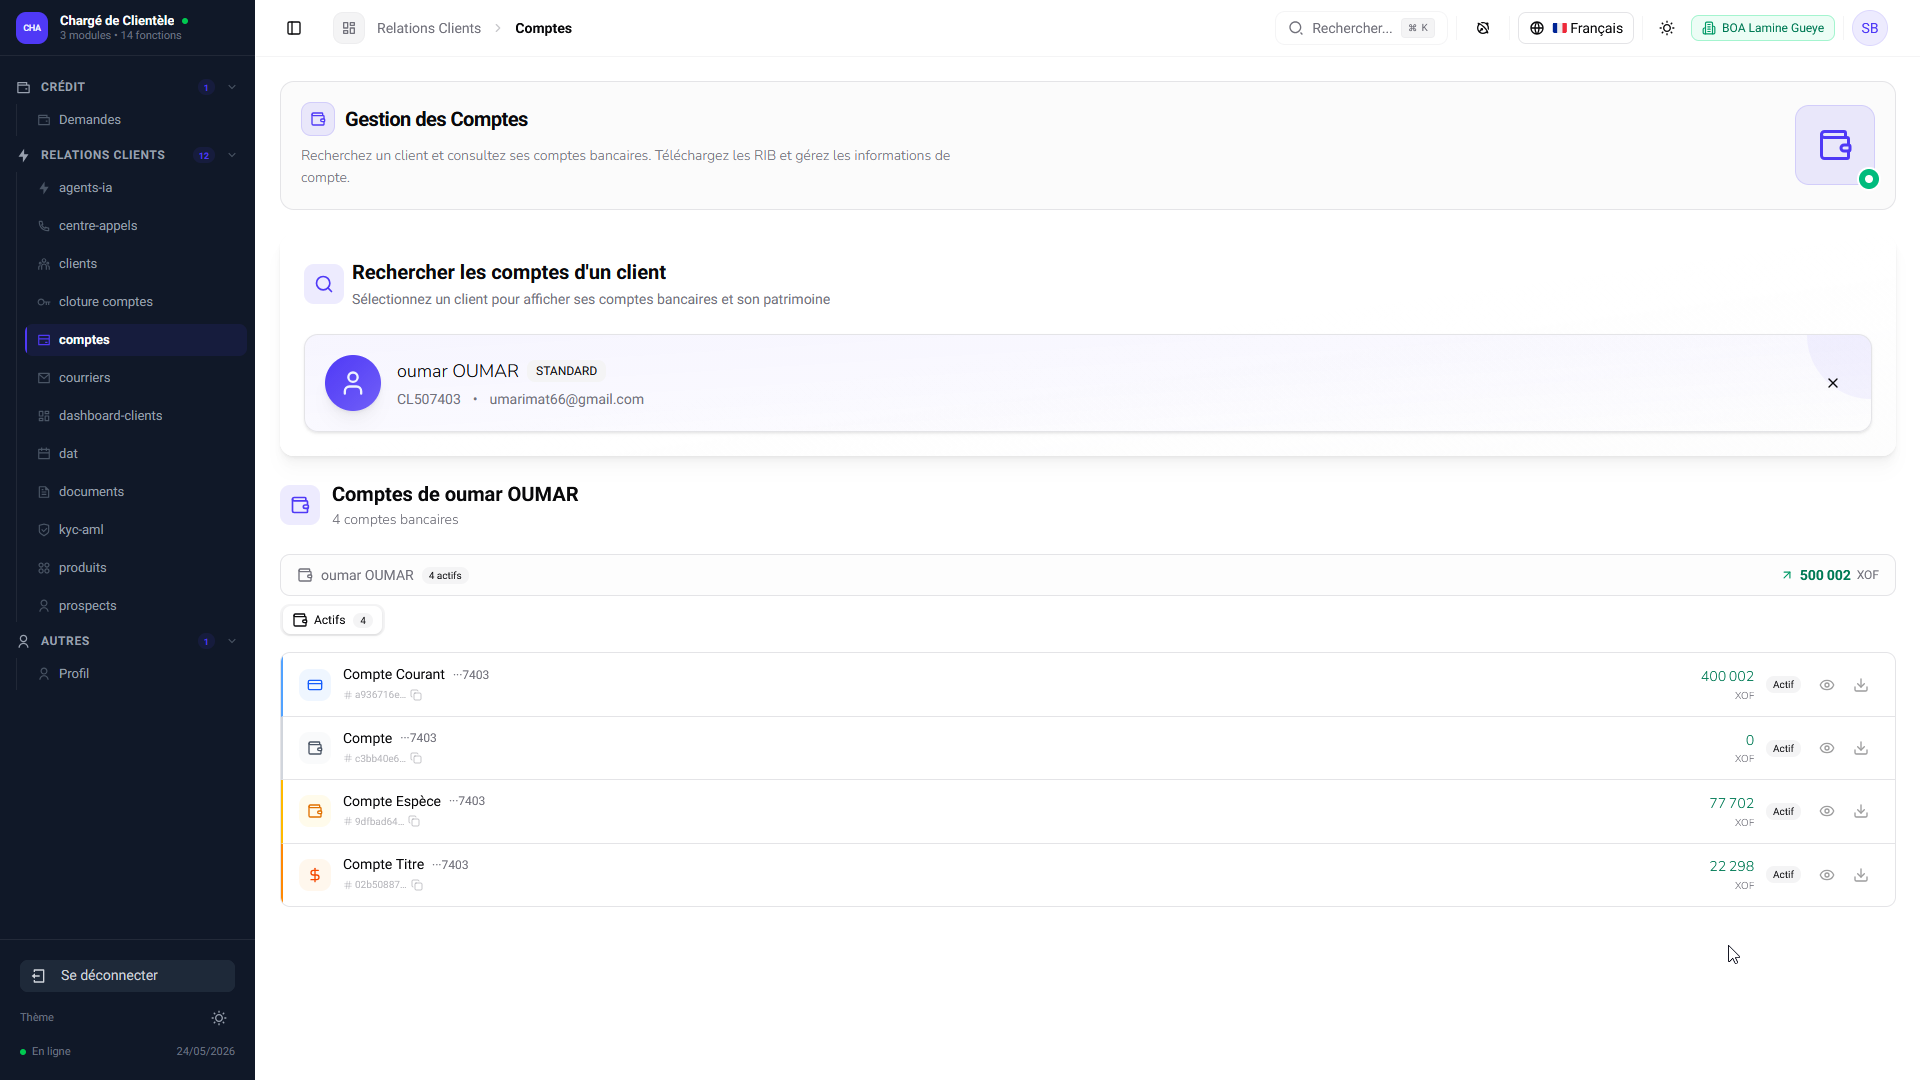
\includegraphics[width=0.88\textwidth]{images/contenu/chapitre-4/gestion_comptes.png}
    \caption{Consultation des comptes bancaires d'un client}
    \label{fig:gestion_comptes}
\end{figure}

\subsection{Agent IA relation client}

L'agent IA relation client facilite l'accès aux informations client à travers
une interrogation en langage naturel. Après sélection du client, le chargé de
clientèle peut poser des questions sur les comptes, les transactions, les
produits bancaires ou le statut KYC/AML. Cette fonctionnalité soutient surtout
la \textbf{détection des risques par l'IA}, notamment le risque de churn, en
rendant les informations utiles plus accessibles.
La figure~\ref{fig:agent_ia_relations} montre l'intégration de cet assistant
dans l'environnement de travail du chargé de clientèle.

\begin{figure}[H]
    \centering
    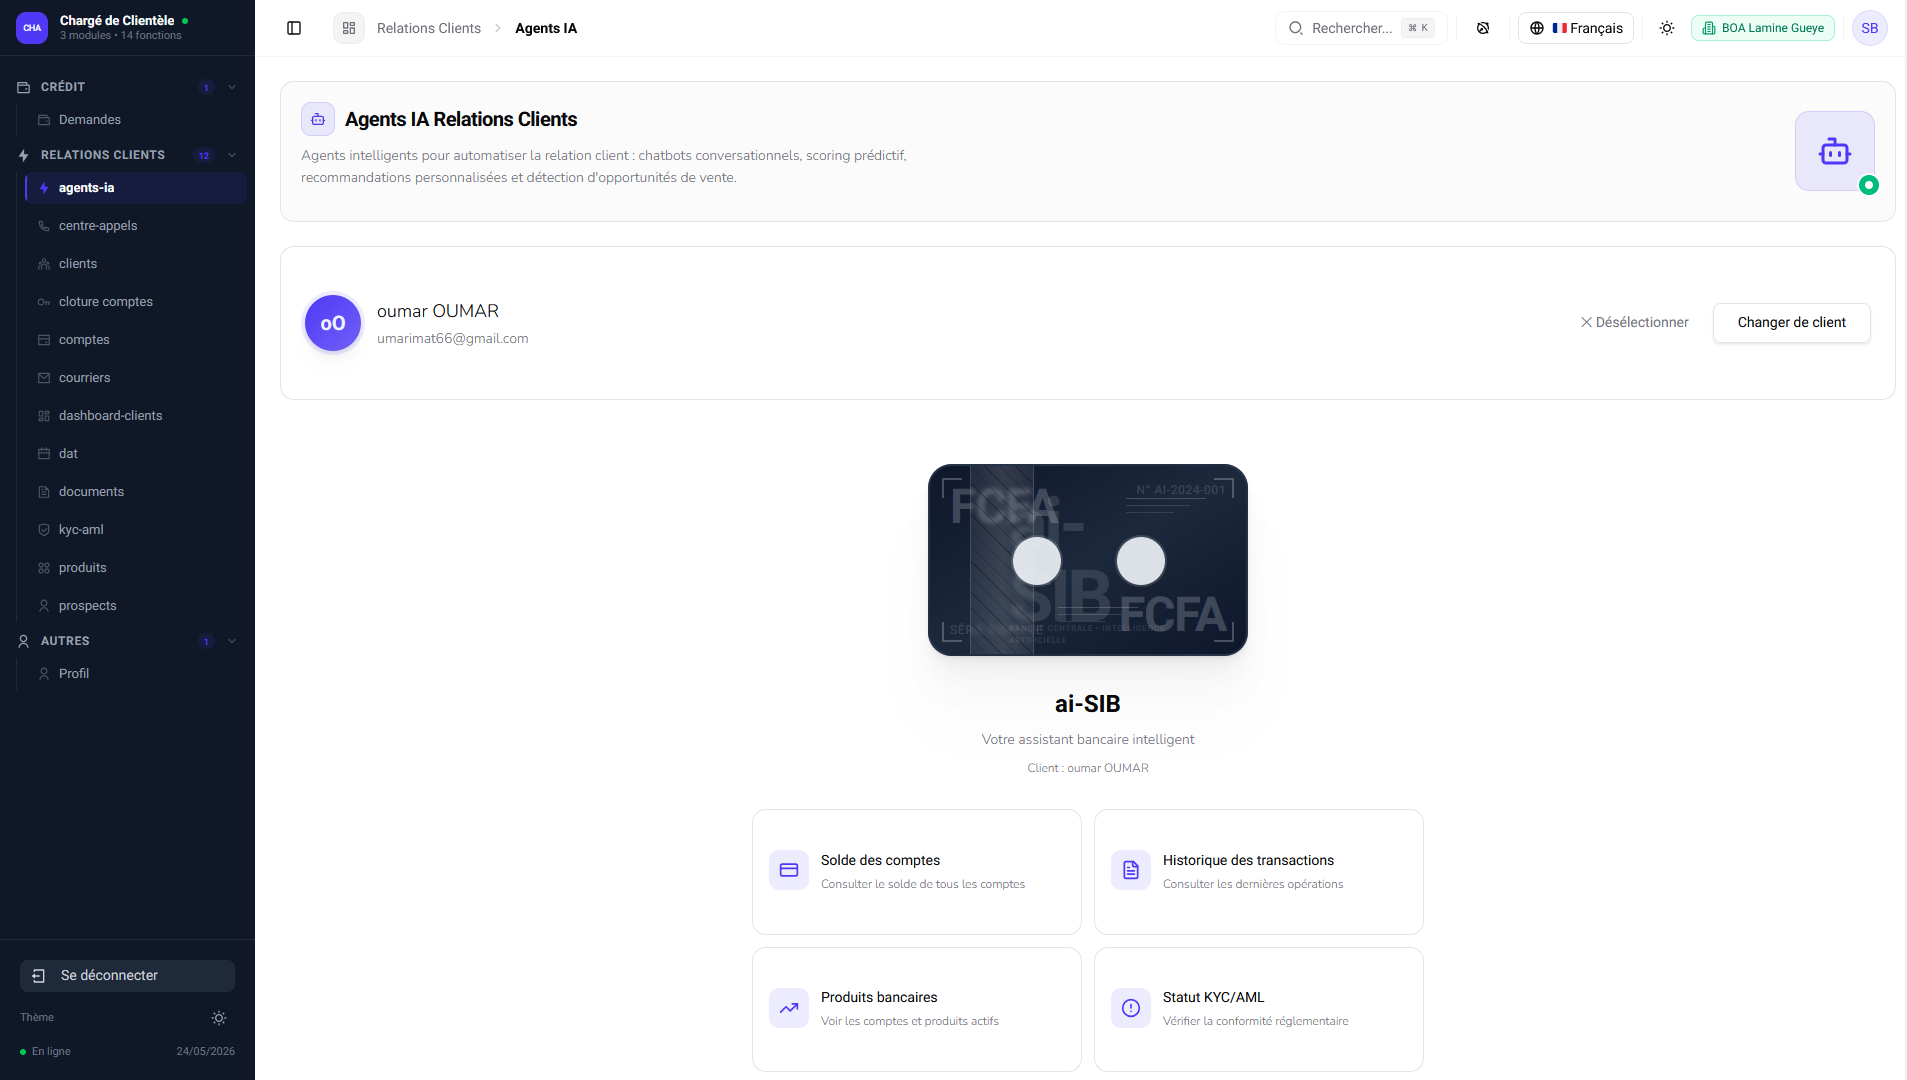
\includegraphics[width=0.88\textwidth]{images/contenu/chapitre-4/agent_ia_relations.png}
    \caption{Agent IA d'interrogation des données client (ai-SIB)}
    \label{fig:agent_ia_relations}
\end{figure}

\subsection{Gestion des prospects}

La gestion des prospects couvre le suivi du cycle commercial avant la conversion
en client. Elle présente les prospects dans un pipeline, avec leur étape
d'avancement, leur priorité, leur score IA et leur date de création. Cette
fonctionnalité permet au chargé de clientèle de prioriser ses actions et
matérialise directement l'objectif de \textbf{gestion des prospects avec
pipeline de conversion et scoring automatique}. La
figure~\ref{fig:gestion_prospects} présente le résultat obtenu pour cette
fonctionnalité centrale du module Relation Client.

\begin{figure}[H]
    \centering
    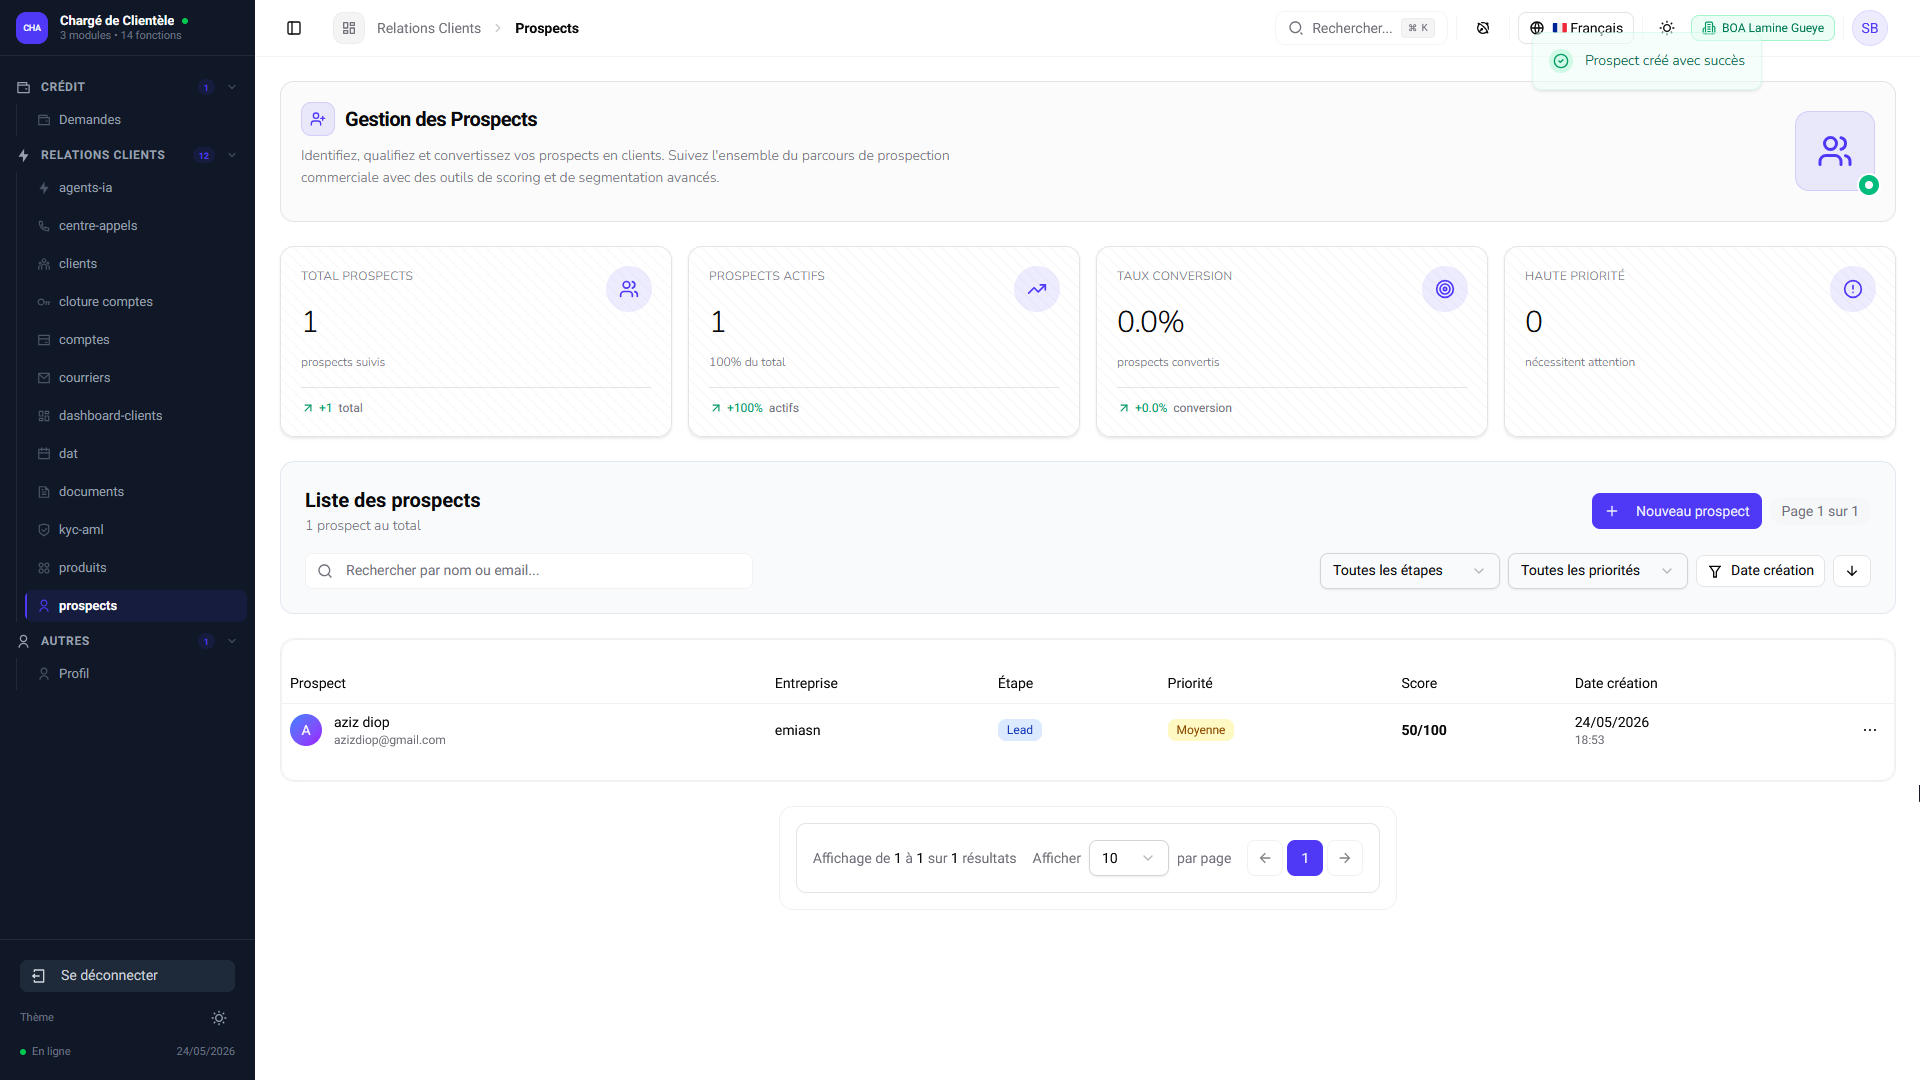
\includegraphics[width=0.88\textwidth]{images/contenu/chapitre-4/gestion_prospects.png}
    \caption{Pipeline de gestion des prospects avec score IA}
    \label{fig:gestion_prospects}
\end{figure}

% ─────────────────────────────────────────────────
\section{Résultats côté SGI}

Le module \textbf{SGI} couvre les opérations d'investissement : portefeuilles,
cotations BRVM et passage d'ordres. Comme pour la Relation Client, les captures
ne sont pas présentées comme de simples écrans isolés ; elles servent à illustrer
les fonctionnalités livrées et leur rôle dans le parcours d'investissement. Les
résultats sont organisés autour de quatre éléments : une vue de pilotage, une
consultation des cotations, une analyse des palmarès de titres et une gestion
détaillée des portefeuilles. Même si l'analyse détaillée du chapitre précédent
s'est concentrée sur le passage d'ordres afin de limiter le périmètre de
conception, ces interfaces sont présentées ici comme des résultats
complémentaires du module SGI, car elles soutiennent la prise de décision avant
la soumission d'un ordre.

\subsection{Tableau de bord SGI}

Le tableau de bord SGI fournit une vue synthétique de l'activité
d'investissement. Il permet de suivre les encours, les portefeuilles, les ordres
en attente et les principaux indicateurs de pilotage. Il donne ainsi une vision
agrégée du module avant d'accéder au détail des portefeuilles. La
figure~\ref{fig:dashboard_sgi} illustre ce tableau de bord de synthèse.

\begin{figure}[H]
    \centering
    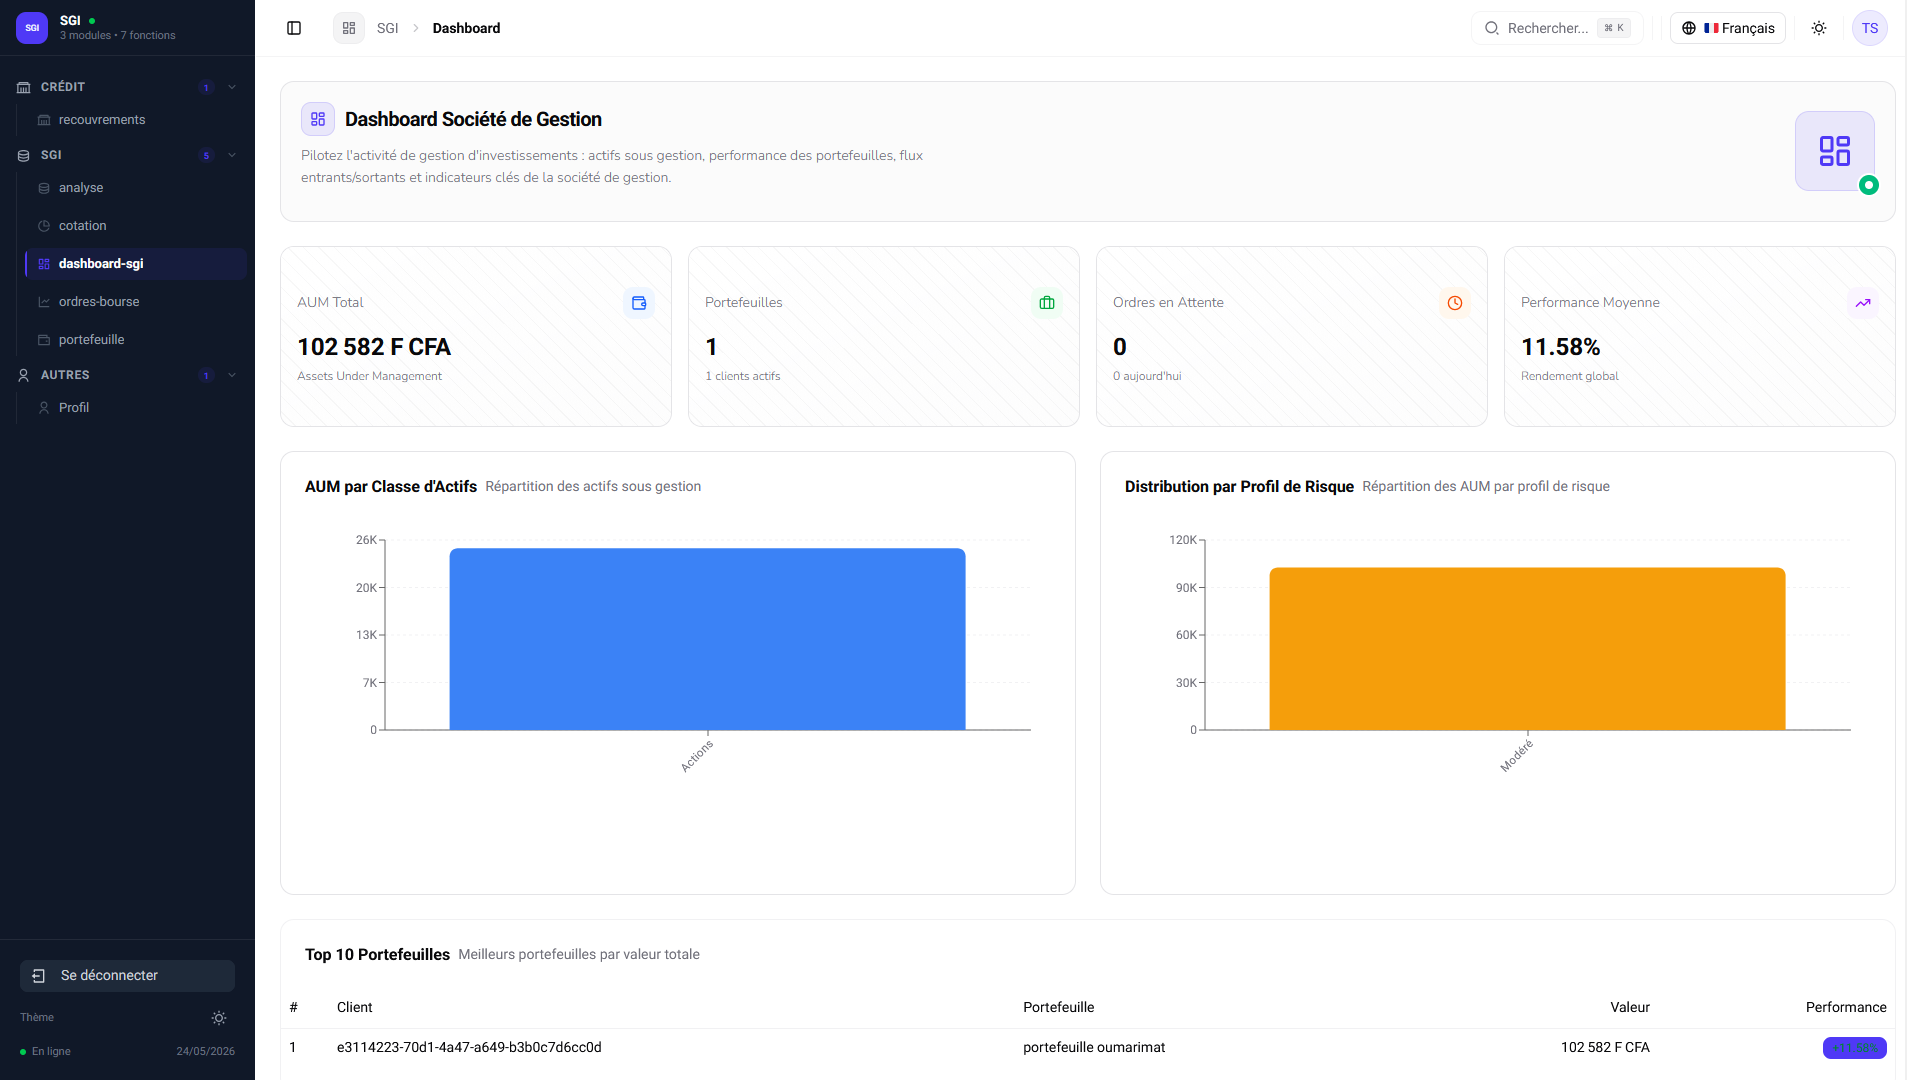
\includegraphics[width=0.88\textwidth]{images/contenu/chapitre-4/dashboard_sgi.png}
    \caption{Tableau de bord global de la Société de Gestion}
    \label{fig:dashboard_sgi}
\end{figure}

\subsection{Cotations BRVM}

La fonctionnalité de cotations permet de consulter les instruments cotés sur la
BRVM, notamment les actions et les obligations \cite{brvm_actions}. Elle fournit les informations
nécessaires à la prise de décision : ticker, dénomination, prix courant,
variation et volume. Cette base de cotation sert de support au passage d'ordres.
La figure~\ref{fig:cotations_brvm} présente l'écran de suivi des instruments de
marché.

\begin{figure}[H]
    \centering
    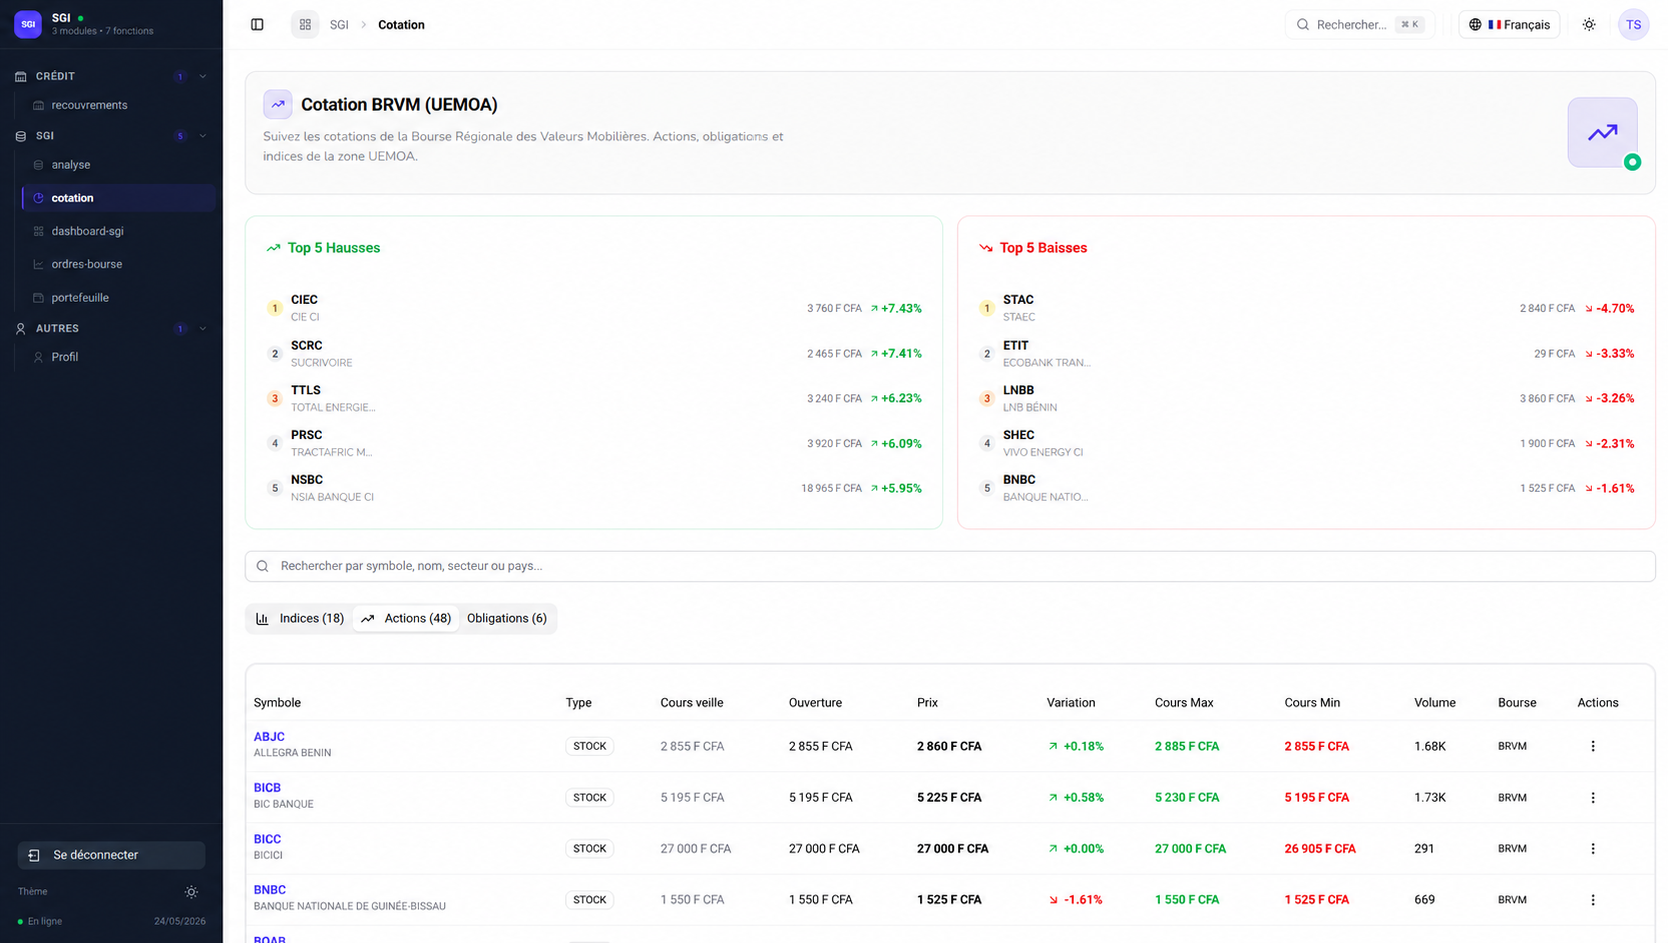
\includegraphics[width=0.88\textwidth]{images/contenu/chapitre-4/cotations_brvm.png}
    \caption{Liste des cotations BRVM et fiche d'un instrument}
    \label{fig:cotations_brvm}
\end{figure}

\subsection{Analyse et palmarès des titres}

En complément de la consultation des cotations, le module SGI propose une page
d'analyse permettant de comparer les performances des titres sur une période
sélectionnée. L'utilisateur peut filtrer les résultats par horizon temporel
(jour, semaine, mois, trimestre, année) et visualiser les meilleures et les plus
faibles performances \cite{brvm_actions}. Cette fonctionnalité aide le gestionnaire à repérer les
tendances du marché et à disposer d'une lecture synthétique avant la prise de
décision. La figure~\ref{fig:palmares_titres} illustre cette vue de palmarès.

\begin{figure}[H]
    \centering
    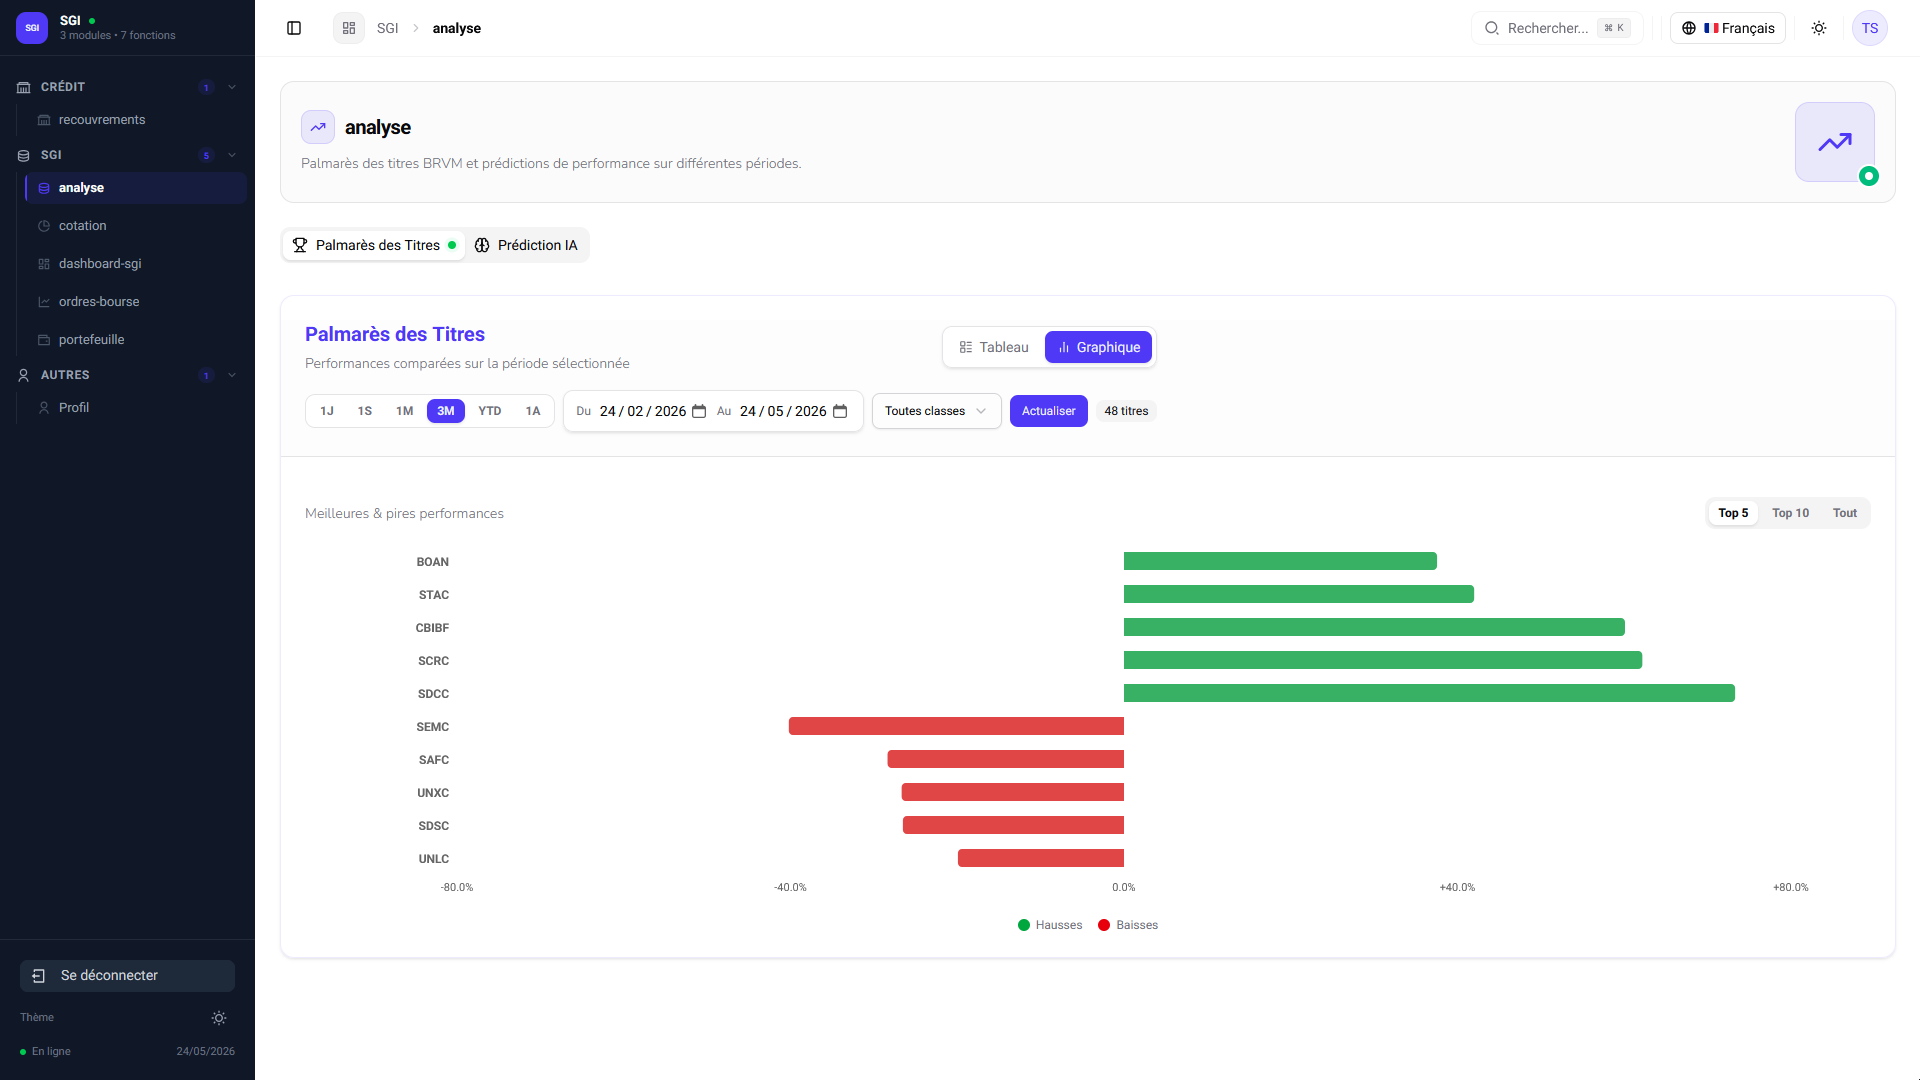
\includegraphics[width=0.88\textwidth]{images/contenu/chapitre-4/palmares.png}
    \caption{Analyse des palmarès des titres BRVM}
    \label{fig:palmares_titres}
\end{figure}

\subsection{Liste des portefeuilles}

La liste des portefeuilles permet au gestionnaire SGI de suivre les
portefeuilles dont il a la charge. Le système présente les informations utiles :
client titulaire, valorisation, profil de risque, composition par actif et
historique des ordres. Cette fonctionnalité complète le tableau de bord SGI par
une lecture plus détaillée et illustre le \textbf{suivi des achats et ventes
d'actions et d'obligations}. La figure~\ref{fig:liste_portefeuilles} montre la
liste des portefeuilles suivis par la SGI.

\begin{figure}[H]
    \centering
    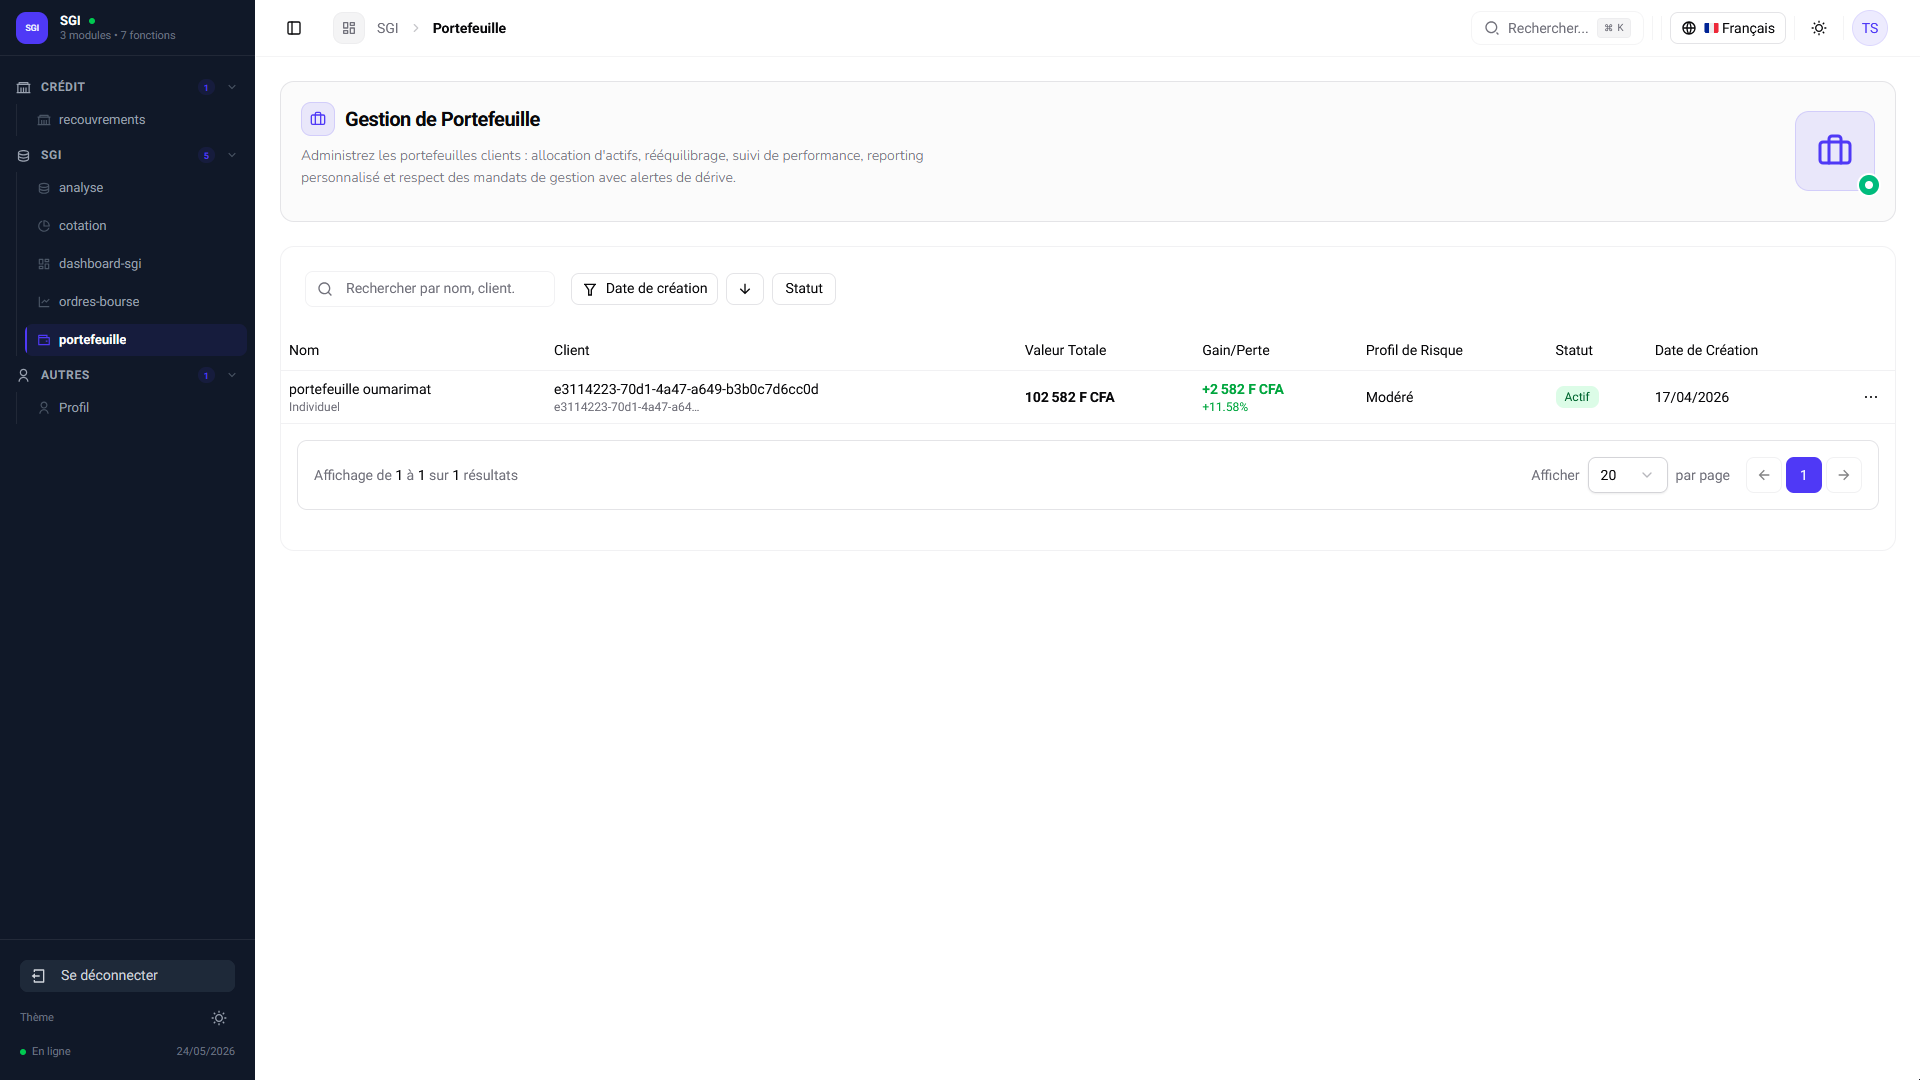
\includegraphics[width=0.88\textwidth]{images/contenu/chapitre-3/liste_portefeuilles}
    \caption{Liste des portefeuilles gérés par la SGI}
    \label{fig:liste_portefeuilles}
\end{figure}

Les interfaces complémentaires du parcours client SGI, notamment la
consultation d'un portefeuille et la saisie d'un ordre, sont prévues en
annexe~\ref{ann:interfaces-client-sgi} afin de compléter les résultats
présentés dans ce chapitre.

% ─────────────────────────────────────────────────
\section{Synthèse de la couverture des objectifs}

Les sections précédentes ont présenté les fonctionnalités réalisées à travers
les interfaces des modules Relation Client et SGI. Il convient à présent de
rapprocher ces résultats des objectifs spécifiques définis au chapitre~1, afin
de vérifier la couverture du périmètre retenu pour le projet. Le
tableau~\ref{tab:couverture_objectifs} synthétise cette correspondance.

\begin{table}[H]
\centering
\caption{Synthèse des objectifs couverts par la réalisation}
\label{tab:couverture_objectifs}
\footnotesize
\renewcommand{\arraystretch}{1.12}
\begin{tabular}{|p{0.55cm}|p{5.0cm}|p{7.05cm}|}
\hline
\textbf{N°} & \textbf{Objectif spécifique} & \textbf{Résultat obtenu} \\ \hline
1 & Tableau de bord Relation Client & Indicateurs de pilotage adaptés aux utilisateurs. \\ \hline
2 & Gestion des prospects & Pipeline commercial et scoring IA. \\ \hline
3 & Vue 360° client & Informations, comptes et produits regroupés. \\ \hline
4 & Dématérialisation des documents & Consultation et téléchargement de documents, dont le RIB. \\ \hline
5 & Suivi KYC du client & Consultation des données KYC/AML. \\ \hline
6 & Détection du churn par l'IA & Estimation du risque de départ client. \\ \hline
7 & Consultation des portefeuilles & Valorisation et composition des portefeuilles SGI. \\ \hline
8 & Cotations et passage d'ordres & Cotations, palmarès et suivi des opérations. \\ \hline
\end{tabular}
\end{table}
\newpage{}
% ─────────────────────────────────────────────────
\section{Analyse critique de la réalisation}

Cette section résume les acquis, les limites et les évolutions prioritaires de
la réalisation, en lien avec la qualité logicielle \cite{iso25010} et la
sécurité applicative \cite{owasp_asvs}.

\subsection{Points forts}

\begin{description}[itemsep=1pt,parsep=0pt]
    \item[Centralisation métier.] I-SIB regroupe Relation Client et SGI dans une
          même plateforme, ce qui améliore l'accès aux informations utiles et la
          continuité des parcours.
    \item[Architecture modulaire.] Le découpage en microservices
          \cite{fowler_microservices} facilite l'évolution progressive de la
          solution et l'isolation des responsabilités.
    \item[Sécurité et traçabilité.] Keycloak \cite{keycloak_docs} centralise
          l'authentification, tandis que RabbitMQ \cite{rabbitmq_docs} soutient
          la traçabilité des actions sensibles.
    \item[Apport de l'IA.] Le scoring des prospects, la détection du churn et la
          segmentation apportent une aide à la priorisation et à la décision.
\end{description}

\subsection{Points faibles et limites}

\begin{description}[itemsep=1pt,parsep=0pt]
    \item[Périmètre encore incomplet.] La plateforme couvre un ensemble large de
          besoins, mais toutes les fonctionnalités et toutes les connexions avec
          les autres modules bancaires ne sont pas encore finalisées.
    \item[Données réelles à intégrer.] Les cotations BRVM restent simulées et
          doivent être remplacées par un flux officiel pour une exploitation
          opérationnelle.
    \item[IA à consolider.] Les modèles devront être évalués et améliorés avec
          des données réelles afin de confirmer leur pertinence métier.
    \item[Passage en production à préparer.] L'environnement de validation
          présenté au chapitre précédent permet les tests actuels, mais l'audit
          de sécurité et l'observabilité avec Zipkin \cite{zipkin_docs} doivent
          être renforcés avant une mise en production.
\end{description}

\subsection{Perspectives d'amélioration}

Les perspectives prioritaires concernent l'achèvement des intégrations avec les
autres modules, le raccordement à un flux BRVM officiel, l'amélioration de l'IA,
l'industrialisation du passage en production et l'ouverture mobile.

% ─────────────────────────────────────────────────
\section*{Conclusion}
\phantomsection
\addcontentsline{toc}{section}{Conclusion}

Ce chapitre a présenté les principaux résultats de la réalisation à travers les
interfaces des modules Relation Client et SGI. Les écrans illustrés montrent la
prise en charge du suivi client, de la gestion des prospects, des portefeuilles,
des cotations et de l'analyse des titres. La synthèse des objectifs confirme
ainsi la couverture du périmètre retenu. L'analyse critique souligne néanmoins
que l'intégration complète avec les autres modules, l'accès à des données
réelles et la préparation de la production constituent les prochaines étapes de
consolidation d'I-SIB.

\chapter*{Conclusion générale}
\phantomsection
\addcontentsline{toc}{chapter}{Conclusion générale}
\markboth{Conclusion générale}{Conclusion générale}

Ce mémoire avait pour objectif de concevoir et de réaliser une solution bancaire
intelligente capable de rapprocher la gestion de la relation client et les services
d'investissement. À travers la plateforme \textbf{I-SIB}, le travail réalisé a
cherché à proposer une solution modulaire, sécurisée et évolutive, adaptée aux
besoins d'un environnement bancaire moderne.

La démarche adoptée a permis d'analyser les besoins, de définir les exigences
fonctionnelles et non fonctionnelles, puis de concevoir une architecture fondée
sur des microservices, une passerelle API, des services métier spécialisés et des
mécanismes de sécurité et de traçabilité. Afin de garder une étude maîtrisée,
l'analyse détaillée s'est concentrée sur deux fonctionnalités représentatives :
la gestion des prospects et le passage d'ordres.

Les résultats obtenus montrent que les principaux objectifs du projet sont
couverts. Le module Relation Client centralise les informations client, facilite
le suivi des prospects, intègre le scoring et la détection du churn. Le module
SGI permet la consultation des portefeuilles, le suivi des cotations BRVM,
l'analyse des titres et le suivi des opérations d'investissement. Ces résultats
montrent l'intérêt d'une plateforme unifiée pour améliorer la continuité entre
les parcours commerciaux, bancaires et d'investissement. La plateforme réalisée
a également été déployée dans un environnement de validation sur un VPS
AlmaLinux, où les évolutions peuvent être testées progressivement après
redéploiement.

Certaines limites demeurent cependant : les cotations BRVM restent simulées, les
modèles d'IA devront être améliorés avec des données réelles et les connexions
avec tous les modules bancaires ne sont pas finalisées. Le passage de
l'environnement de validation à la production nécessitera également davantage
de tests, un audit de sécurité approfondi et une observabilité plus complète.
Les perspectives portent donc sur l'intégration de flux de marché officiels,
l'industrialisation de la production, la haute disponibilité et l'ouverture
future vers le mobile ou le multilingue.

En définitive, ce projet a permis de démontrer la faisabilité d'une plateforme
unifiée combinant relation client, services d'investissement, architecture
modulaire et intelligence artificielle. Il constitue une base solide pour la
poursuite du développement d'I-SIB et son adaptation progressive aux besoins
réels des institutions financières.

% ─────────────────────────────────────────────────
%  RÉFÉRENCES BIBLIOGRAPHIQUES
% ─────────────────────────────────────────────────
\renewcommand{\bibname}{Références bibliographiques}
\begin{thebibliography}{99}
\phantomsection
\addcontentsline{toc}{chapter}{Références bibliographiques}

\bibitem{fowler_microservices}
M. Fowler et J. Lewis, \textit{Microservices}, martinfowler.com, 2014.
Disponible sur : \url{https://martinfowler.com/articles/microservices.html}

\bibitem{iso25010}
ISO/IEC, \textit{ISO/IEC 25010: Systems and software Quality Requirements and Evaluation (SQuaRE) -- Product quality model}.
Disponible sur : \url{https://iso25000.com/index.php/en/iso-25000-standards/iso-25010}

\bibitem{owasp_asvs}
OWASP Foundation, \textit{Application Security Verification Standard (ASVS)}.
Disponible sur : \url{https://owasp.org/www-project-application-security-verification-standard/}

\bibitem{fatf_digital_id}
FATF, \textit{Guidance on Digital Identity}, Financial Action Task Force, 2020.
Disponible sur : \url{https://www.fatf-gafi.org/en/publications/Financialinclusionandnpoissues/Digital-identity-guidance.html}

\bibitem{brvm_actions}
BRVM, \textit{Marché des actions}, Bourse Régionale des Valeurs Mobilières.
Disponible sur : \url{https://www.brvm.org/fr/marche-des-actions}

\bibitem{esp_officiel}
École Supérieure Polytechnique de Dakar, \textit{Site institutionnel de l'ESP}.
Disponible sur : \url{https://esp.sn/}

\bibitem{innov4africa_officiel}
INNOV4AFRICA, \textit{Site institutionnel de l'entreprise}.
Disponible sur : \url{https://innov4africa.com/}

\bibitem{nextjs_docs}
Vercel, \textit{Next.js Documentation}.
Disponible sur : \url{https://nextjs.org/docs}

\bibitem{typescript_docs}
Microsoft, \textit{TypeScript Handbook}.
Disponible sur : \url{https://www.typescriptlang.org/docs/handbook/}

\bibitem{spring_boot_docs}
VMware Tanzu, \textit{Spring Boot Reference Documentation}.
Disponible sur : \url{https://docs.spring.io/spring-boot/}

\bibitem{spring_gateway_docs}
VMware Tanzu, \textit{Spring Cloud Gateway Reference Documentation}.
Disponible sur : \url{https://docs.spring.io/spring-cloud-gateway/reference/}

\bibitem{spring_eureka_docs}
VMware Tanzu, \textit{Spring Cloud Netflix Eureka Documentation}.
Disponible sur : \url{https://docs.spring.io/spring-cloud-netflix/reference/}

\bibitem{keycloak_docs}
Keycloak, \textit{Keycloak Documentation}.
Disponible sur : \url{https://www.keycloak.org/documentation}

\bibitem{postgresql_docs}
PostgreSQL Global Development Group, \textit{PostgreSQL Documentation}.
Disponible sur : \url{https://www.postgresql.org/docs/}

\bibitem{redis_docs}
Redis, \textit{Redis Documentation}.
Disponible sur : \url{https://redis.io/docs/}

\bibitem{rabbitmq_docs}
Broadcom, \textit{RabbitMQ Documentation}.
Disponible sur : \url{https://www.rabbitmq.com/docs}

\bibitem{minio_docs}
MinIO, \textit{MinIO Object Store Documentation}.
Disponible sur : \url{https://min.io/docs/minio/linux/index.html}

\bibitem{rasa_docs}
Rasa, \textit{Rasa Documentation}.
Disponible sur : \url{https://rasa.com/docs/}

\bibitem{zipkin_docs}
OpenZipkin, \textit{Zipkin Documentation}.
Disponible sur : \url{https://zipkin.io/pages/documentation.html}

\bibitem{docker_docs}
Docker Inc., \textit{Docker Documentation}.
Disponible sur : \url{https://docs.docker.com/}

\bibitem{docker_compose_docs}
Docker Inc., \textit{Docker Compose Documentation}.
Disponible sur : \url{https://docs.docker.com/compose/}

\bibitem{jacobson_oose}
I. Jacobson, M. Christerson, P. Jonsson et G. Övergaard, \textit{Object-Oriented Software Engineering: A Use Case Driven Approach}, Addison-Wesley, 1992.

\end{thebibliography}

% ─────────────────────────────────────────────────
%  ANNEXES
% ─────────────────────────────────────────────────
\appendix
\renewcommand{\chaptername}{Annexe}

% ═════════════════════════════════════════════════
%  ANNEXE A – Interfaces complémentaires du parcours client SGI
% ═════════════════════════════════════════════════
\chapter{Interfaces complémentaires du parcours client SGI}
\markboth{Interfaces complémentaires SGI}{Interfaces complémentaires SGI}
\label{ann:interfaces-client-sgi}

Le chapitre~4 a présenté les résultats du module SGI du point de vue du
gestionnaire (tableau de bord, cotations, portefeuilles). La présente annexe
complète cette vue en illustrant le parcours tel qu'il est vécu par le
\textbf{client} : depuis la consultation de son portefeuille jusqu'à la
soumission d'un ordre d'investissement.

Trois interfaces sont présentées :
\begin{itemize}
  \item la consultation du portefeuille client
        (figure~\ref{fig:ann_portefeuille_client}) ;
  \item la fiche détaillée d'un titre coté sur la BRVM
        (figure~\ref{fig:ann_detail_titre}) ;
  \item le formulaire de saisie d'un ordre d'achat ou de vente
        (figure~\ref{fig:ann_passage_ordre}).
\end{itemize}

\section{Consultation du portefeuille}

L'interface de consultation du portefeuille permet au client de visualiser la
composition et la valorisation de ses actifs avant toute décision
d'investissement. Elle affiche les positions détenues, leur cours actuel et
la performance associée.

\begin{figure}[H]
    \centering
    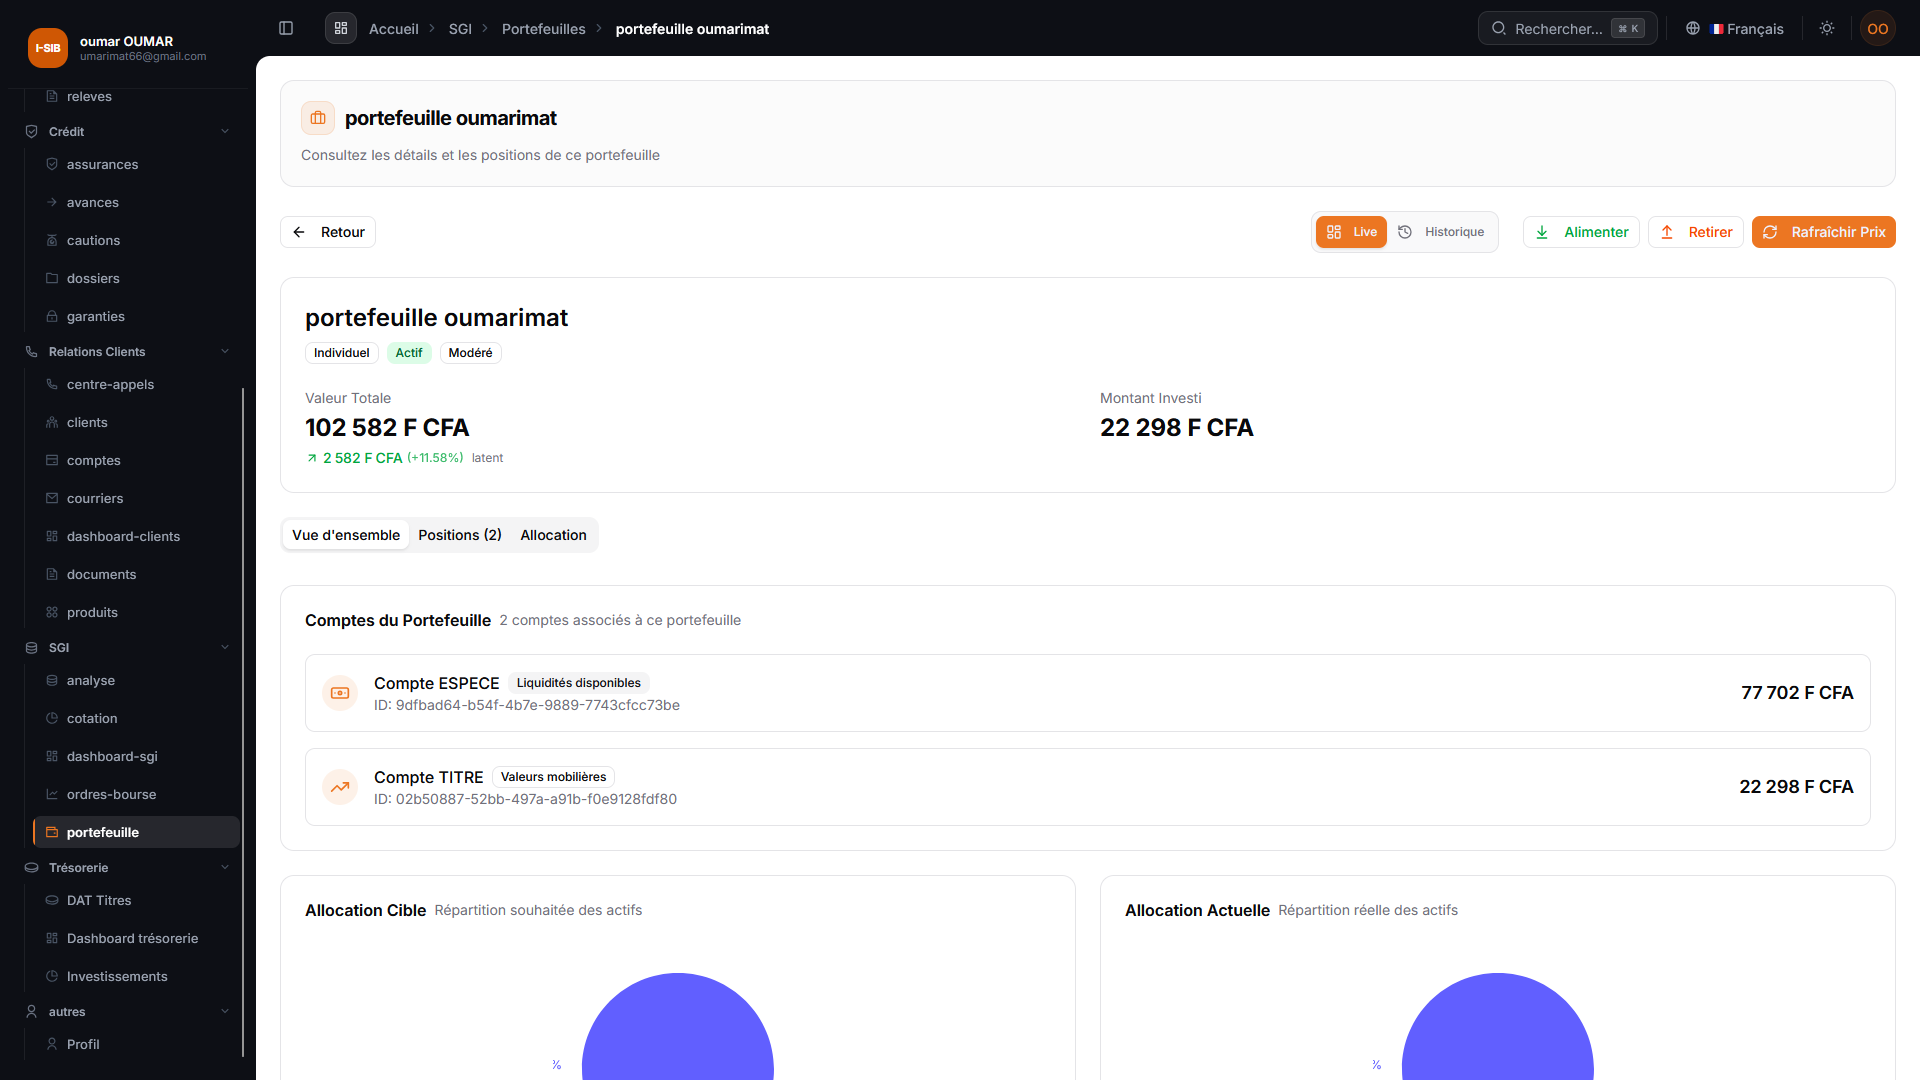
\includegraphics[width=0.88\textwidth]{images/annexes/annexe_a/annexe_a_portefeuille_client.png}
    \caption{Consultation du portefeuille côté client}
    \label{fig:ann_portefeuille_client}
\end{figure}

\section{Consultation d'un titre}

La fiche d'un titre présente les informations nécessaires à la prise de
décision : cours actuel, variation, volume échangé, historique de cotation
et caractéristiques de l'instrument. Cette vue précède la saisie d'un ordre.

\begin{figure}[H]
    \centering
    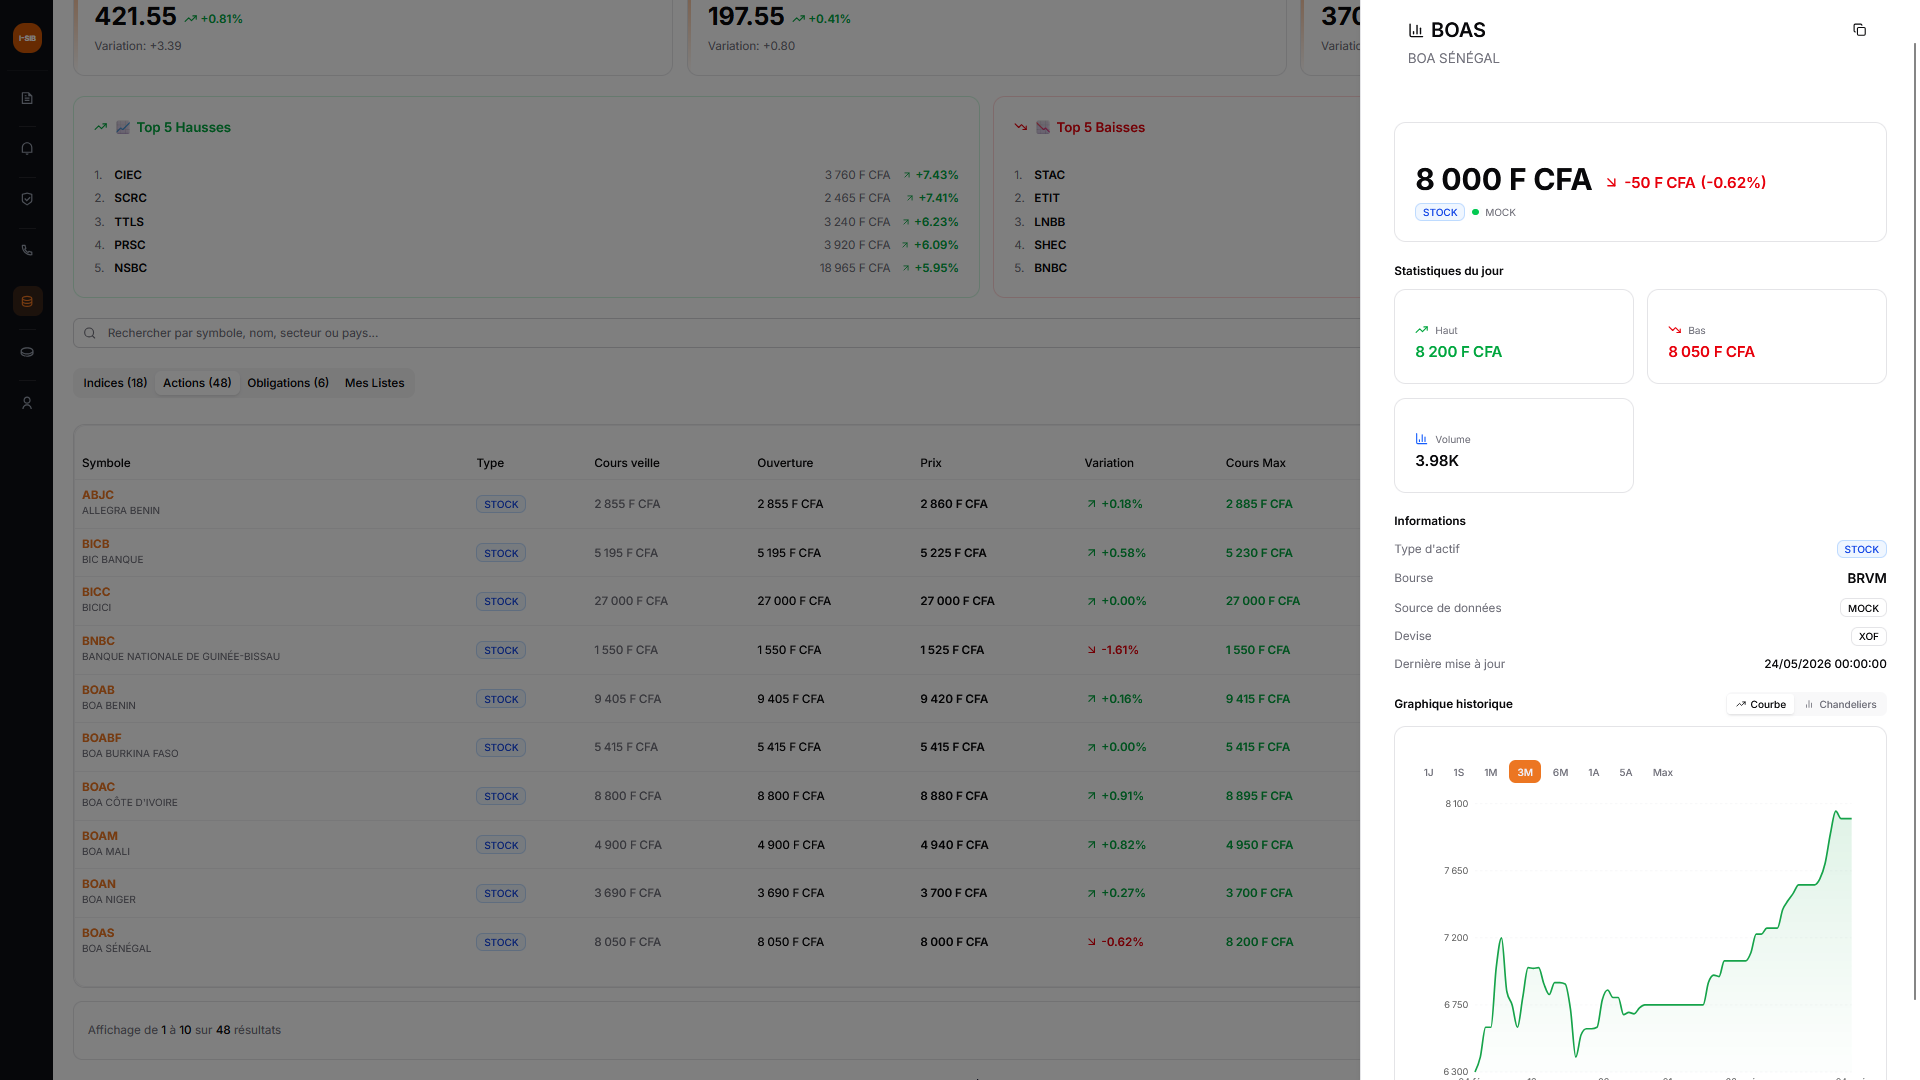
\includegraphics[width=0.88\textwidth]{images/annexes/annexe_a/annexe_a_detail_titre_client.png}
    \caption{Fiche détaillée d'un titre coté sur la BRVM}
    \label{fig:ann_detail_titre}
\end{figure}

\section{Saisie d'un ordre}

Le formulaire de passage d'ordre permet au client de soumettre une intention
d'achat ou de vente sur un instrument coté. Une fois soumis, l'ordre suit le
workflow de traitement décrit au chapitre~2 : saisie, prise en charge par
l'équipe SGI, validation puis exécution.

\begin{figure}[H]
    \centering
    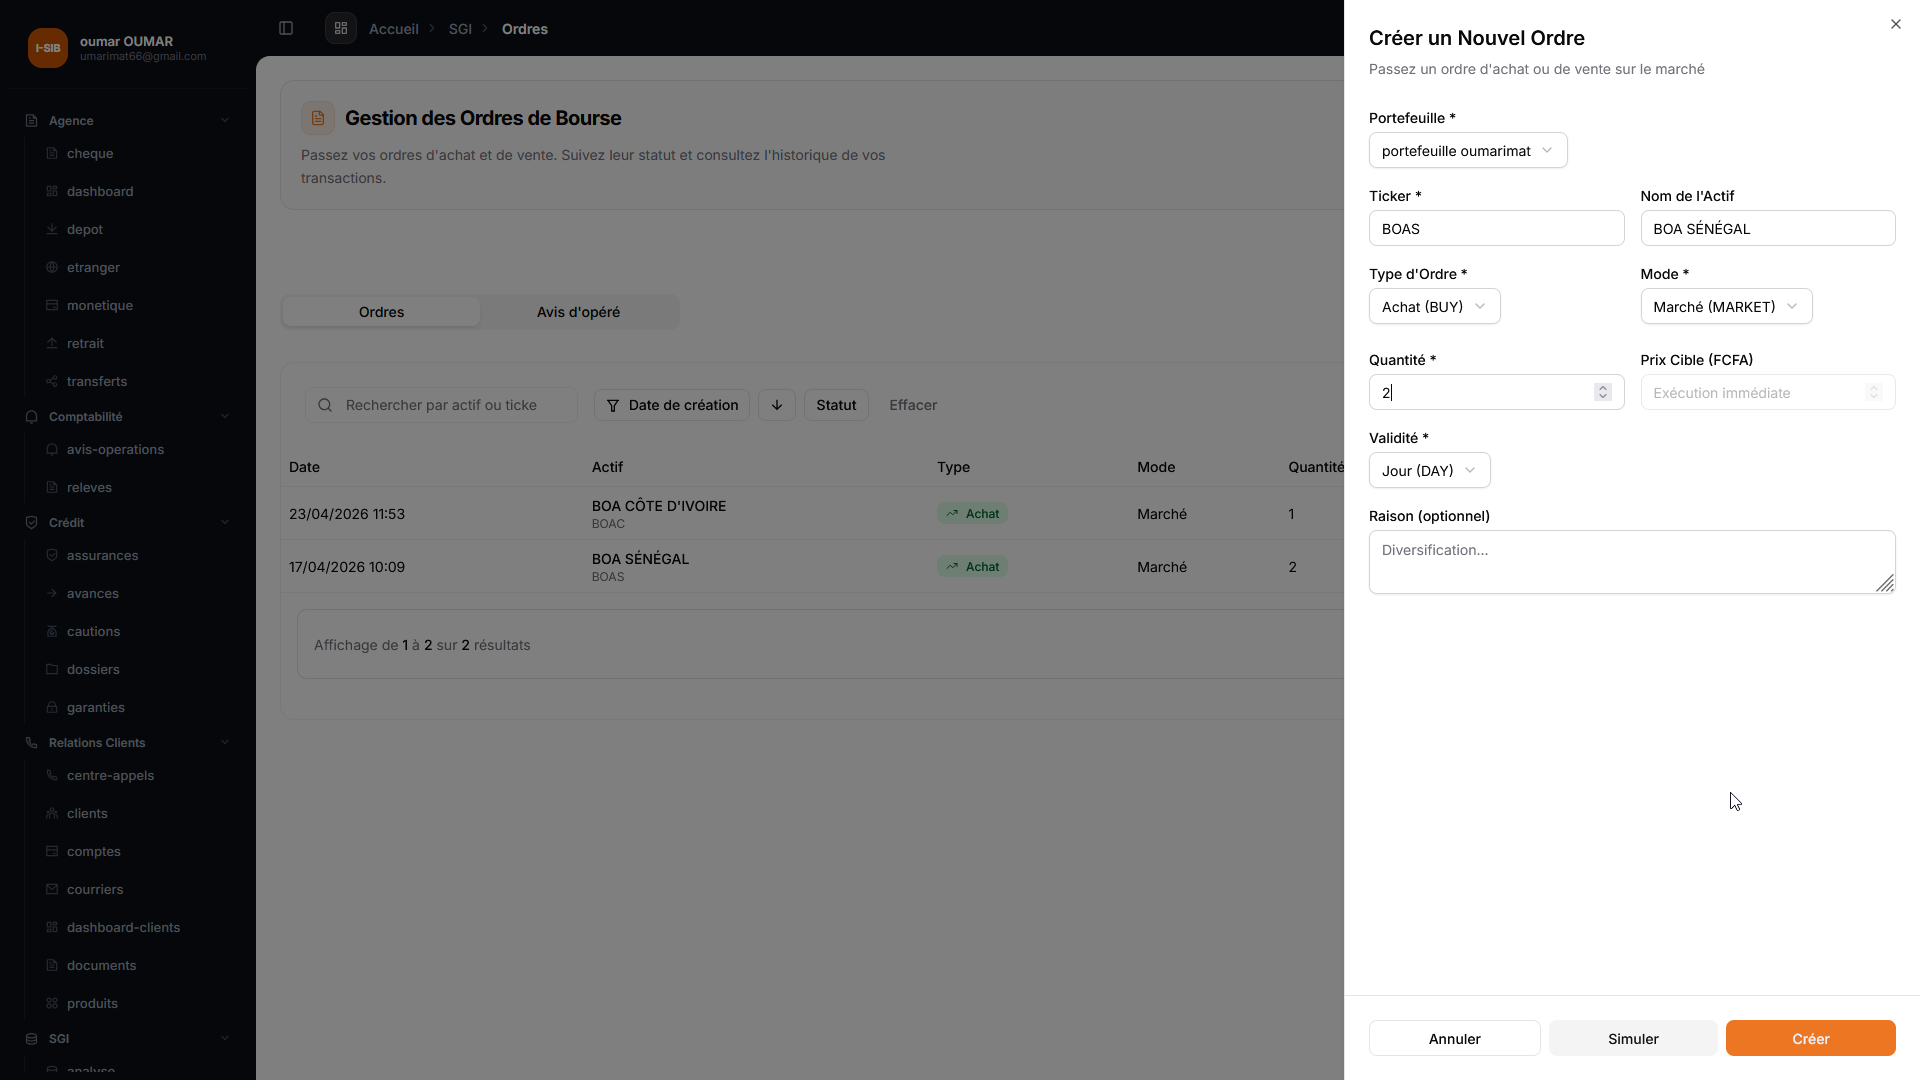
\includegraphics[width=0.88\textwidth]{images/annexes/annexe_a/annexe_a_passage_ordre_client.png}
    \caption{Formulaire de saisie d'un ordre d'investissement}
    \label{fig:ann_passage_ordre}
\end{figure}

% ═════════════════════════════════════════════════
%  ANNEXE B – Pièces de recette fonctionnelle
% ═════════════════════════════════════════════════
\chapter{Pièces de recette fonctionnelle}
\markboth{Pièces de recette fonctionnelle}{Pièces de recette fonctionnelle}
\label{ann:recette-fonctionnelle}

Cette annexe regroupe les preuves de tests fonctionnels réalisés sur le
parcours de gestion des prospects, fonctionnalité détaillée aux chapitres~2
et~3. L'objectif est de montrer que les deux scénarios critiques du cycle
commercial fonctionnent de bout en bout dans l'application déployée.

Deux scénarios sont documentés :
\begin{itemize}
  \item la création d'un prospect avec calcul automatique du score IA
        (figure~\ref{fig:recette_creation}) ;
  \item la conversion d'un prospect en client avec segmentation ML, création
        du compte et envoi de l'email de bienvenue
        (figure~\ref{fig:recette_conversion}).
\end{itemize}

Le tableau~\ref{tab:pieces_recette_annexe} récapitule les résultats attendus
pour chaque scénario.

\begin{table}[H]
\centering
\caption{Scénarios de recette documentés}
\label{tab:pieces_recette_annexe}
\small
\renewcommand{\arraystretch}{1.3}
\begin{tabular}{|p{4.5cm}|p{5.5cm}|p{4.0cm}|}
\hline
\textbf{Scénario} & \textbf{Résultat attendu} & \textbf{Référence} \\ \hline
Création d'un prospect &
Prospect enregistré avec score initial calculé par le modèle IA &
Figure~\ref{fig:recette_creation} \\ \hline
Conversion d'un prospect en client &
Client créé, prospect marqué converti et email de bienvenue envoyé &
Figure~\ref{fig:recette_conversion} \\ \hline
\end{tabular}
\end{table}

\section{Création d'un prospect}

La création d'un prospect déclenche automatiquement le calcul du score IA via
le service de scoring. Le chargé de clientèle peut alors visualiser le score
et la probabilité de conversion attribués au nouveau prospect directement
depuis l'interface du pipeline commercial.

\begin{emplacementcapture}{Capture à insérer : \texttt{annexe\_b\_creation\_prospect.png}}
Résultat observé après création d'un prospect et calcul du score.
\end{emplacementcapture}
\captionof{figure}{Résultat de la création d'un prospect avec score IA}
\label{fig:recette_creation}

\section{Conversion d'un prospect en client}

La conversion déclenche le workflow complet décrit au chapitre~3 : appel au
service de segmentation ML pour déterminer le type de client, création du
compte via le Customer Service, initialisation du scoring churn par le
Dashboard Service et envoi d'un email de bienvenue contenant les identifiants
de connexion. La figure~\ref{fig:recette_conversion} montre le résultat
observé à l'issue de ce processus.

\begin{emplacementcapture}{Capture à insérer : \texttt{annexe\_b\_conversion\_prospect.png}}
Résultat observé après conversion d'un prospect qualifié en client.
\end{emplacementcapture}
\captionof{figure}{Résultat de la conversion d'un prospect en client}
\label{fig:recette_conversion}

% ═════════════════════════════════════════════════
%  ANNEXE C – Validation du déploiement sur VPS AlmaLinux
% ═════════════════════════════════════════════════
\chapter{Validation du déploiement sur VPS AlmaLinux}
\markboth{Validation du déploiement}{Validation du déploiement}
\label{ann:validation-deploiement}

Cette annexe rassemble les preuves visuelles de l'environnement de validation
mentionné au chapitre~3. Elle permet de vérifier que l'ensemble des
composants de la plateforme I-SIB sont correctement déployés et opérationnels
sur le serveur AlmaLinux utilisé pour la recette.

Trois éléments sont documentés :
\begin{itemize}
  \item l'état des conteneurs Docker via l'interface Portainer
        (figure~\ref{fig:ann_portainer}) ;
  \item l'enregistrement des microservices dans le registre Eureka
        (figure~\ref{fig:ann_eureka}) ;
  \item l'historique de redéploiement attestant du processus itératif
        de mise à jour (figure~\ref{fig:ann_redeploiement}).
\end{itemize}

\section{Services conteneurisés}

La vue Portainer permet de vérifier que l'ensemble des conteneurs Docker des
quatre stacks (infra, core, module, office) sont actifs et opérationnels sur
le serveur de validation.

\begin{emplacementcapture}{Capture à insérer : \texttt{annexe\_c\_portainer\_conteneurs.png}}
Vue Portainer des conteneurs I-SIB actifs sur le VPS AlmaLinux.
\end{emplacementcapture}
\captionof{figure}{Conteneurs Docker actifs sur le VPS AlmaLinux}
\label{fig:ann_portainer}

\section{Enregistrement des services}

Le tableau Eureka confirme que chaque microservice est correctement enregistré
auprès du registre de services et prêt à recevoir des requêtes acheminées par
la passerelle API.

\begin{emplacementcapture}{Capture à insérer : \texttt{annexe\_c\_eureka\_services.png}}
Tableau Eureka montrant les services applicatifs enregistrés et disponibles.
\end{emplacementcapture}
\captionof{figure}{Services enregistrés dans le registre Eureka}
\label{fig:ann_eureka}

\section{Redéploiement progressif}

L'historique de redéploiement atteste du processus itératif de mise à jour des
services sur le serveur de validation, en cohérence avec la démarche
incrémentale adoptée pour le projet.

\begin{emplacementcapture}{Capture à insérer : \texttt{annexe\_c\_pipeline\_redeploiement.png}}
Historique attestant d'un redéploiement de validation sur le VPS.
\end{emplacementcapture}
\captionof{figure}{Historique de redéploiement sur le serveur de validation}
\label{fig:ann_redeploiement}



\end{document}
